%%
%% This is file `sample-sigconf.tex',
%% generated with the docstrip utility.
%%
%% The original source files were:
%%
%% samples.dtx  (with options: `all,proceedings,bibtex,sigconf')
%% 
%% IMPORTANT NOTICE:
%% 
%% For the copyright see the source file.
%% 
%% Any modified versions of this file must be renamed
%% with new filenames distinct from sample-sigconf.tex.
%% 
%% For distribution of the original source see the terms
%% for copying and modification in the file samples.dtx.
%% 
%% This generated file may be distributed as long as the
%% original source files, as listed above, are part of the
%% same distribution. (The sources need not necessarily be
%% in the same archive or directory.)
%%
%%
%% Commands for TeXCount
%TC:macro \cite [option:text,text]
%TC:macro \citep [option:text,text]
%TC:macro \citet [option:text,text]
%TC:envir table 0 1
%TC:envir table* 0 1
%TC:envir tabular [ignore] word
%TC:envir displaymath 0 word
%TC:envir math 0 word
%TC:envir comment 0 0
%%
%% The first command in your LaTeX source must be the \documentclass
%% command.
%%
%% For submission and review of your manuscript please change the
%% command to \documentclass[manuscript, screen, review]{acmart}.
%%
%% When submitting camera ready or to TAPS, please change the command
%% to \documentclass[sigconf]{acmart} or whichever template is required
%% for your publication.
%%
%%
\documentclass[sigconf]{acmart}
%\documentclass[sigconf,anonymous,review]{acmart}

%%
%% \BibTeX command to typeset BibTeX logo in the docs
\AtBeginDocument{%
  \providecommand\BibTeX{{%
    Bib\TeX}}}

%% Rights management information.  This information is sent to you
%% when you complete the rights form.  These commands have SAMPLE
%% values in them; it is your responsibility as an author to replace
%% the commands and values with those provided to you when you
%% complete the rights form.
% \setcopyright{acmlicensed}
% \copyrightyear{2018}
% \acmYear{2018}
% \acmDOI{XXXXXXX.XXXXXXX}
%% These commands are for a PROCEEDINGS abstract or paper.
% \acmConference[Conference acronym 'XX]{Make sure to enter the correct
%   conference title from your rights confirmation email}{June 03--05,
%   2018}{Woodstock, NY}
%%
%%  Uncomment \acmBooktitle if the title of the proceedings is different
%%  from ``Proceedings of ...''!
%%
%%\acmBooktitle{Woodstock '18: ACM Symposium on Neural Gaze Detection,
%%  June 03--05, 2018, Woodstock, NY}
% \acmISBN{978-1-4503-XXXX-X/18/06}


\usepackage{tikz}
\usepackage{subfigure}
\usepackage{graphicx} 
\usepackage{multirow}
\usepackage{pgfplots} 
\usepackage{pgfplotstable}
\usepackage{lineno}
\usepackage{wrapfig}

\usepackage{enumitem}

\usepackage{listings}
\usepackage{geometry}
\lstset{
    basicstyle=\ttfamily,
    literate={,}{,}1
}
\usepackage{rotating}

\PassOptionsToPackage{prologue,dvipsnames,svgnames}{xcolor}
%\usepackage[prologue,dvipsnames]{xcolor}
\usepackage{graphicx}
\setlength{\fboxsep}{1pt}
\usepackage{xcolor}
\usepackage[many]{tcolorbox} 
\definecolor{bblue}{HTML}{4F81BD}
\definecolor{rred}{HTML}{C0504D}
\pgfplotsset{compat=1.11,
        /pgfplots/ybar legend/.style={
        /pgfplots/legend image code/.code={%
        %\draw[##1,/tikz/.cd,yshift=-0.25em]
                %(0cm,0cm) rectangle (3pt,0.8em);},
        \draw[##1,/tikz/.cd,bar width=3pt,yshift=-0.2em,bar shift=0pt]
                plot coordinates {(0cm,0.8em)};},
},
}

%%
%% Submission ID.
%% Use this when submitting an article to a sponsored event. You'll
%% receive a unique submission ID from the organizers
%% of the event, and this ID should be used as the parameter to this command.
%%\acmSubmissionID{123-A56-BU3}

%%
%% For managing citations, it is recommended to use bibliography
%% files in BibTeX format.
%%
%% You can then either use BibTeX with the ACM-Reference-Format style,
%% or BibLaTeX with the acmnumeric or acmauthoryear sytles, that include
%% support for advanced citation of software artefact from the
%% biblatex-software package, also separately available on CTAN.
%%
%% Look at the sample-*-biblatex.tex files for templates showcasing
%% the biblatex styles.
%%

%%
%% The majority of ACM publications use numbered citations and
%% references.  The command \citestyle{authoryear} switches to the
%% "author year" style.
%%
%% If you are preparing content for an event
%% sponsored by ACM SIGGRAPH, you must use the "author year" style of
%% citations and references.
%% Uncommenting
%% the next command will enable that style.
%%\citestyle{acmauthoryear}


%%
%% end of the preamble, start of the body of the document source.
\begin{document}

%%
%% The "title" command has an optional parameter,
%% allowing the author to define a "short title" to be used in page headers.
\title[Self-Regularization with Latent Space Explanations for Controllable LLM-based Classification]{Self-Regularization with Latent Space Explanations for \\ Controllable LLM-based Classification}
%\title[Towards Interpretable LLM-based Classification: Self-Regularization with Latent Space Explanations]{Towards Interpretable LLM-based Classification: Self-Regularization with Latent Space Explanations}


%%
%% The "author" command and its associated commands are used to define
%% the authors and their affiliations.
%% Of note is the shared affiliation of the first two authors, and the
%% "authornote" and "authornotemark" commands
%% used to denote shared contribution to the research.
\author{Xuansheng Wu\textsuperscript{1}, Wenhao Yu\textsuperscript{2}, Xiaoming Zhai\textsuperscript{1}, Ninghao Liu\textsuperscript{1}}
%\orcid{0000-0002-7816-7658}
\affiliation{%
  \institution{\textsuperscript{1}University of Georgia\,\,\,\,\textsuperscript{2}Tencent AI Lab, Seattle}
  \country{\textsuperscript{1}\{xuansheng.wu, xiaoming.zhai, ninghao.liu\}@uga.edu\,\,\,\,\textsuperscript{2}wenhaowyu@global.tencent.com}
}


% \author{Xuansheng Wu}
% \orcid{0000-0002-7816-7658}
% \affiliation{%
%   \institution{University of Georgia}
%   \city{Athens}
%   \state{Georgia}
%   \country{United States}
% }
% \email{xuansheng.wu@uga.edu}

% \author{Wenhao Yu}
% %\orcid{0000-0002-7816-7658}
% \affiliation{%
%   \institution{Tencent AI Lab, Seattle}
% }
% \email{wenhaowyu@global.tencent.com}

% \author{Xiaoming Zhai}
% \orcid{0000-0003-4519-1931}
% \affiliation{%
%   \institution{University of Georgia}
% }
% \email{xiaoming.zhai@uga.edu}
% \author{Ninghao Liu}
% %\orcid{0000-0002-7816-7658}
% \affiliation{%
%   \institution{University of Georgia}
% }
% \email{ninghao.liu@uga.edu}

%%
%% By default, the full list of authors will be used in the page
%% headers. Often, this list is too long, and will overlap
%% other information printed in the page headers. This command allows
%% the author to define a more concise list
%% of authors' names for this purpose.
\renewcommand{\shortauthors}{Wu et al.}

%%
%% The abstract is a short summary of the work to be presented in the
%% article.
\begin{abstract}
Modern text classification methods heavily rely on contextual embeddings from large language models (LLMs). 
Compared to human-engineered features, these embeddings provide automatic and effective representations for classification model training. 
However, they also introduce a challenge: we lose the ability to manually remove \emph{unintended features}, such as sensitive or task-irrelevant features, to guarantee regulatory compliance or improve the generalizability of classification models. This limitation arises because LLM embeddings are opaque and difficult to interpret. 
In this paper, we propose a novel framework to identify and regularize unintended features in the LLM latent space.
Specifically, we first pre-train a sparse autoencoder (SAE) to extract interpretable features from LLM latent spaces. 
To ensure the SAE can capture task-specific features, we further fine-tune it on task-specific datasets. 
In training the classification model, we propose a simple and effective regularizer, by minimizing the similarity between the classifier weights and the identified unintended feature, to remove the impacts of these unintended features toward classification. 
We evaluate the proposed framework on three real-world tasks, including toxic chat detection, reward modeling, and disease diagnosis. 
Results show that the proposed framework can significantly improve the classifier's generalizability by regularizing those features that are not semantically correlated to each task. 
This work pioneers controllable text classification on LLM latent spaces by leveraging interpreted features to address generalizability, fairness, and privacy challenges. We will release our code and data once accepted.

%Text classification plays a key role in many real-world applications, such as search engines, spam filtering, and content moderation, where automated systems categorize textual data for specific tasks.  
%Modern text classification models rely on contextual representations generated by large language models (LLMs), which significantly improve classifier performance by providing rich semantic information. 
%In many real-world applications, developers may expect to exclude the use of some features, called \textit{unintended features}. 
%It is common in scenarios where developers aim to improve generalizability by excluding shortcut features or to ensure compliance with fairness and privacy regulations by regularizing the usage of sensitive features. 
% However, achieving this goal in embedding-based text classification is challenging, as the inputs of modern text classifiers are text representations generated by large language models (LLMs), which are typically unexplainable to humans. 
% Therefore, developers cannot identify and exclude these unintended features from the LLM latent space with straightforward feature engineering strategies. 
% Modern text classification models rely on contextual representations generated by large language models (LLMs), which significantly improve classifier performance by providing rich semantic information. 
% In many real-world applications, developers may expect to exclude the use of some features, called \textit{unintended features}. 
% However, achieving this goal in embedding-based text classification is challenging, as these LLM-generated embeddings are inherently unexplainable, making it difficult for developers to identify and exclude unintended features using straightforward feature engineering strategies.


% Modern text classification methods heavily rely on contextual embeddings from large language models (LLMs). 
% Compared to human-engineered features, these embeddings provide automatic and effective representations for classification model training. 
% However, they also introduce a challenge: we lose the ability to manually remove \emph{unintended features}, such as sensitive or task-irrelevant features, to guarantee regulatory compliance or improve generalizability of classification models. This limitation arises because LLM embeddings are opaque and difficult to interpret. 
% % However, achieving this goal in embedding-based classifiers is challenging because LLM-generated embeddings are inherently opaque, making it impossible to identify and remove unintended features through conventional feature-engineering techniques. 
% In this paper, we propose a novel framework to identify and regularize unintended features in the LLM latent space. %, leveraging the capabilities of LLMs themselves. 
% Specifically, we first pre-train a sparse autoencoder (SAE) to extract interpretable features from LLM latent spaces. 
% To ensure the SAE can capture task-specific features, we further fine-tune it on task-specific datasets. 
% % During this process, we allow the inactivated features (``dead'' features) to reconstruct the residuals of the normal features. 
% In training the classification model, we propose a simple and effective regularizer, by minimizing the similarity between the classifier weights and the identified unintended feature, to remove the impacts of these unintended features toward classification. 
% We evaluate the proposed framework on three real-world tasks, including toxic chat detection, reward modeling, and disease diagnosis. 
% Results show that the proposed self-regularization framework can significantly improve the classifier's generalizability by regularizing those features that are not semantically correlated to each task. 
% This work pioneers controllable text classification on LLM latent spaces by leveraging interpreted features to address generalizability, fairness, and privacy challenges.
\end{abstract}

%%
%% The code below is generated by the tool at http://dl.acm.org/ccs.cfm.
%% Please copy and paste the code instead of the example below.
%%

\begin{CCSXML}
<ccs2012>
   <concept>
       <concept_id>10010147.10010257.10010321.10010337</concept_id>
       <concept_desc>Computing methodologies~Regularization</concept_desc>
       <concept_significance>500</concept_significance>
       </concept>
   <concept>
       <concept_id>10010147.10010178.10010179</concept_id>
       <concept_desc>Computing methodologies~Natural language processing</concept_desc>
       <concept_significance>500</concept_significance>
       </concept>
   <concept>
       <concept_id>10010147.10010257.10010293.10010319</concept_id>
       <concept_desc>Computing methodologies~Learning latent representations</concept_desc>
       <concept_significance>500</concept_significance>
       </concept>
 </ccs2012>
\end{CCSXML}

%\ccsdesc[500]{Computing methodologies~Regularization}
\ccsdesc[500]{Computing methodologies~Natural language processing}
%\ccsdesc[500]{Computing methodologies~Learning latent representations}


%%
% Keywords. The author(s) should pick words that accurately describe
% the work being presented. Separate the keywords with commas.
\keywords{Sparse Autoencoder, Text Classification, Interpretability, Large Language Model, Regularization}
%% A "teaser" image appears between the author and affiliation
%% information and the body of the document, and typically \textbf{Span}s the
%% page.
% \begin{teaserfigure}
%   \includegraphics[width=\textwidth]{sampleteaser}
%   \caption{Seattle Mariners at Spring Training, 2010.}
%   \Description{Enjoying the baseball game from the third-base
%   seats. Ichiro Suzuki preparing to bat.}
%   \label{fig:teaser}
% \end{teaserfigure}

% \received{20 February 2007}
% \received[revised]{12 March 2009}
% \received[accepted]{5 June 2009}

%%
%% This command processes the author and affiliation and title
%% information and builds the first part of the formatted document.
\maketitle


\section{Introduction}
\vspace{-0.1cm}
Large language models (LLMs) have demonstrated remarkable proficiency in handling diverse user queries and tasks through dialogues~\cite{liu2024deepseek, dubey2024llama}. Yet, many real-world applications still rely heavily on text classification models for specific and well-defined objectives, such as search engines~\cite{zhu2023large}, spam filtering~\cite{tusher2024email}, and content moderation~\cite{markov2023holistic}. With the advent of powerful LLMs, these classification models have shifted away from manually engineered features toward using LLM-generated contextual embeddings as input. Unlike traditional features designed by humans, LLM-generated embeddings capture richer semantic information in high-dimensional latent spaces, often providing substantially improved performance over feature-based approaches.


In numerous scenarios of classifier training, there is a pressing need to explicitly exclude or control certain features, referred to as \textbf{unintended features}. 
For instance, task-irrelevant attributes (e.g., the hospital information or appointment date in disease diagnosis) can bias predictions and degrade the generalizability of the classifier~\cite{zhou2024navigating}. Likewise, sensitive attributes (e.g., demographic data or identifiers) must be shielded from model usage in order to meet fairness, privacy, and regulatory standards~\cite{krishna2022measuring}.
Previously, with conventional \emph{feature-based} classifiers that relied on constructed features (e.g., TF-IDF scores), it was straightforward to ``exclude'' or ``edit out'' unintended features due to their transparent, human-engineered nature~\cite{sun2019mitigating}. 
Unfortunately, the same level of direct control is not readily available with \emph{embedding-based} classifiers, where high-dimensional representations generated by LLMs intermix a broad range of semantic information. 
This opacity makes it difficult to selectively remove or neutralize the impacts of unintended features to the embedding-based classifiers. 
%This request can be easily satisfied if the classifier is built on conventional \emph{feature-based} modeling, where each feature is manually constructed and designed by human experts, such as word frequency or TF-IDF scores~\cite{sun2019mitigating}. 
%While feature-based modeling offers great transparency, it typically performs worse than nowadays \emph{embedding-based} modeling, which benefits from leveraging contextual text representations provided by LLMs. 
\textbf{These scenarios highlight the need for methods to regulate the usage of unintended features within LLM latent spaces.} 

However, achieving this goal presents significant challenges. 
The first challenge is identifying unintended features in the text representations. 
Unlike conventional input spaces where features are explicitly defined, LLM latent spaces implicitly encode features as dense and entangled representations, which are \emph{polysemantic}~\cite{arora2018linear,scherlis2022polysemanticity}. 
Specifically, each dimension of the latent space refers to multiple distinct concepts, making it difficult to understand the meanings of each dimension by simply analyzing their values across different input texts. 
Early works~\cite{hewitt2019structural,chenprobing} try to identify whether an interested feature is encoded in the latent space by using supervised learning, also known as ``probing'', where researchers first collect a dataset of annotated samples clearly with or without the interested feature, and then a probing classifier is trained to predict the existing of interested feature based on LLM-generated embeddings of the input texts. 
They finally conclude that the latent space encoded the interested feature if the probing model achieves high accuracy on this task.
%Yet, this approach is not feasible for our purpose since human experts cannot exhaust all possible unintended features, and even so, it is costly to collect a training dataset for each unintended feature. 
Yet, this approach is not feasible for our purpose since collecting a training dataset for each possible unintended feature is costly. 
Some researchers proposed to break the constraint in an unsupervised manner~\cite{millidge2022singular,dar2023analyzing,wu2024language}, where they learn a set of orthogonal basis vectors of the latent space by using matrix decomposition techniques.  
However, this line of work cannot produce fine-grained features since matrix decomposition techniques limit the maximum number of basis vectors we can learn. 
The second challenge is regularizing text classifiers to avoid relying on unintended features during training. 
While naive feature exclusion strategies~\cite{zafar2017fairness} may remove the direct influence of unintended features, they cannot eliminate indirect correlations between unintended features and model predictions via retained features. 
In conventional feature-based modeling, this bottleneck can be broken by measuring the correlation between the occurrence of the unintended features and model predictions~\cite{zafar2017fairness,quadrianto2017recycling,baharlouei2019r}. 
However, these measurements cannot be estimated effectively and efficiently in the LLM latent spaces.

%In this work, we address these gaps by proposing a self-regularization framework to extract and constrain the use of unintended features in LLM latent spaces. 
In this work, we propose a self-regularization framework to extract and constrain the use of unintended features for text classifier development in the LLM latent space with LLMs. 
Specifically, our framework leverages sparse autoencoders (SAEs)~\cite{makhzani2013k,huben2023sparse} to learn encoded features from the LLM latent space. 
To ensure the sparse autoencoders can learn task-specific features, we propose a novel two-stage training paradigm, where the sparse autoencoders first pre-train on a general corpus, and then fine-tune on the task dataset. 
During fine-tuning, the ``dead'' features (i.e., pre-trained features that have not been activated on the task dataset) are encouraged to reconstruct the residuals of the reconstructions generated by the normal activated features. 
To interpret each learned feature, we collect the most activated input text spans from the task dataset. 
The LLM is prompted to judge whether a learned feature should be classified as an unintended feature according to a human-written guideline and its most activated text spans. 
In addition, we propose to regularize the similarity between the classifier weights and the learned unintended feature vectors to alleviate the indirect impacts of the unintended features on model predictions. 
To this end, the proposed framework can identify unintended features in the LLM latent space and regulate their use in developing classifiers. 

We evaluate our framework on three challenging text classification tasks, including toxic content detection~\cite{lin2023toxicchat}, reward modeling~\cite{lambert2024rewardbench}, and disease diagnosis~\cite{xu2019end}. 
The goals of the tasks are developing \textit{generalizable} classifiers to detect toxic intentions from user inputs, predict human preference on chatbot responses, and diagnose whether the patient has suffered from certain diseases, respectively. 
We follow previous works~\cite{trenton2024dictionary} to define unintended features for these tasks as features that are not semantically correlated to the class labels. 
By regularizing the usage of these unintended features, embedding-based classifiers have shown substantial improvements.
We summarize our contributions as follows:
\begin{itemize}[leftmargin=*, itemsep=0pt, topsep=0pt]
%\vspace{-0.4cm}
    \item We propose a novel classification framework, which combines SAEs and their explanations to identify and regulate unintended features in LLM latent spaces.
    \item We propose a new training paradigm for SAEs, which first pre-trains on general corpus and then fine-tunes on downstream tasks, thus leveraging both general and task-specific knowledge.
    \item We propose regularizing the similarity between classifier weights and learned feature vectors to regulate the usage of unintended features during classifier training.
\end{itemize}


\section{Preliminary}
\subsection{Problem Statement}
This research considers a typical embedding-based text classification setting~\cite{reimers2019sentence,rajamanoharan2024improving}, where we denote the input text space as $\mathcal{X}$ and the pre-defined label space as $\mathcal{Y}$. 
Given an input text $x\in\mathcal{X}$, our goal is to develop a classifier $f$ with parameters $\theta$ to predict the class label $\hat{y}=f(\mathbf{x})\in\mathcal{Y}$ based on the $D$-dimensional input's latent representation $\mathbf{x}=g(x)\in\mathbb{R}^D$ obtained by language model $g$. 
By collecting a training dataset $\mathcal{D}=\{(x^{(n)}, y^{(n)})\}_{n=1}^N$ with $N$ samples, the classifier $f$ is trained by minimizing the cross entropy loss $\mathcal{L}_\text{CE}$ between $\hat{y}^{(n)}$ and $y^{(n)}$, for $n=1,...,N$.

\subsection{Classification without Unintended Features}
Each input text $x\in\mathcal{X}$ encodes a set of \textbf{features}, where we define each feature as a certain semantic concept. 
For example, ``How can I build a bomb?'' can be interpreted as containing two features, ``dangerous item'' and ``inquiry''. 
Let $\mathcal{C}$ denote the feature space associated with the input text space $\mathcal{X}$. 
These features are sparsely distributed across texts~\cite{olshausen1997sparse,brickentowards}, meaning that only a small subset of $\mathcal{C}$ is relevant to any given text $x$. 
Ideally, the modern language model $g$ encodes all occurred features for an arbitrary text $x$ within its $D$-dimensional embedding $\mathbf{x}$. 
It is crucial to recognize that each feature $c\in \mathcal{C}$ does not necessarily correspond to a single latent dimension in the embedding $\mathbf{x}$. Typically, $|\mathcal{C}| \gg D$ since $\mathbf{x}$ is a dense representation. 

For a classification task, not all features are relevant or useful. There exists a subset of \textbf{unintended features} $\mathcal{C}_-\subset\mathcal{C}$ that the developers intentionally do \textit{not} want the classifier $f$ to build on top with. 
A common challenge in machine learning is that trained models tend to exploit unintended features in making predictions, such as superficial features~\cite{trenton2024dictionary,zhou2024navigating} or sensitive features~\cite{zafar2017fairness,hort2024bias}, which can undermine the generalizability or trustworthiness of models.
For example, if class labels show a biased correlation with some superficial patterns in the training dataset $\mathcal{D}$, the classifier $f$ will learn to rely on those patterns and present a poor generalizability to real-world scenarios. 
Usually, whether a feature is unintended or not is decided by human experts, who can define biased or superficial patterns as unintended features and aim to prevent their influence in model establishment. 
However, manual identification is not scalable and is prone to errors.
This work focuses on controlling the use of unintended features in embedding-based text classification without relying on human experts. 


%
%
\section{Methodology}
This section introduces our proposed framework to regularize embedding-based text classifiers, ensuring that no unintended features are used, by leveraging the language model $g$ to interpret its own latent space.
Section~\ref{sec:learn_feature_based_classifier} starts with describing a general regularization framework on conventional \emph{feature-based} text classification settings, where we discuss two challenges to leverage their methods to our \emph{embedding-based} setting.
To overcome the challenges, we first propose identifying unintended features from the LLM latent space by fine-tuning a sparse autoencoder in Section~\ref{sec:SAE}. 
We also propose a regularizing term to limit the usage of unintended features on the embedding-based classifiers in Section~\ref{sec:regularize}. 


\subsection{Regularizing Classifiers against Unintended Features on Feature Space}
\label{sec:learn_feature_based_classifier}
Traditionally, classifiers are developed on top of the feature vectors instead of hidden representations of instances. 
Formally, given the feature space $\mathcal{C}$, the classifier's input is a vector $\mathbf{z}\in\mathbb{R}^{\|\mathcal{C}\|}$, where each element $\mathbf{z}[c]$ is the value of the $c$-th feature. 
One trivial solution to regularize the usage of unintended features is to explicitly exclude them~\cite{kamishima2011fairness}. 
However, this trivial solution can only regularize the direct impact from unintended features $\mathcal{C}_-$ to the class labels $\mathcal{Y}$~\cite{zafar2017fairness}, while the indirect impacts from unintended features to the class labels via those remaining features still maintain. 
Taking the disease diagnosis task as an example, developers consider the patient's gender an unintended feature to satisfy the fairness requests. 
Although we can simply delete the gender feature from the patient profile, some other features may still leak the patient's gender information, such as a history of cervical cancer indicating the patient is a female. 
Another approach to remove both direct and indirect impacts is regularizing the correlation between the model prediction and the values of unintended features~\cite{kamishima2011fairness,zafar2017fairness,huang2019stable}. 
One of the most straightforward measurements is covariance, i.e., 
\begin{equation}
\begin{aligned}
\text{Covar}(\mathbf{z}_-, f(\mathbf{z}_+))\approx \frac{1}{N}\sum_{n=1}^N (\mathbf{z}_-^{(n)}-\bar{\mathbf{z}}_-)\cdot f(\mathbf{z}_+^{(n)}).
\end{aligned}
\label{eq:covar}
\end{equation}
where $\mathbf{z}_+\in\mathbb{R}^{\|\mathcal{C}\|}$ is the purified feature vector with zero values on all unintended features, $\mathbf{z}_-=\mathbf{z}-\mathbf{z}_+$, and $\bar{\mathbf{z}}_-$ is the average values of $\mathbf{z}_-$ over dataset $\mathcal{D}$. 
During the classifier training, one may introduce Equation~\eqref{eq:covar} as a constraint while minimizing the cross-entropy loss $\mathcal{L}_\text{CE}$ to encourage the classifier to make predictions without taking unintended features into account.

However, this approach is not applicable for training classifiers in our embedding-based setting. 
Firstly, the text representations generated from language models are \textbf{not directly explainable}, so we do not have a human-understandable feature space $\mathcal{C}$. 
Thus, human experts cannot manually identify the unintended feature subset or engineer the input feature space. 
Secondly, even if we could identify those unintended features from the latent space, computing the covariance between the model predictions and the unintended features on the embeddings is infeasible (see discussion in Appendix~\ref{appd:training_size}). 
To tackle these challenges, we introduce our framework to extract unintended features from the latent space of language models, and design a method to regularize unintended features when building the classifier $f$.


\begin{figure}
\centerline{\includegraphics[width=1.0\linewidth]{Figures/FineTuneFigure_v4.pdf}}
\vspace{-0.25cm}
\caption{Fine-tuning pre-trained sparse autoencoder $h$ on the classification dataset $\mathcal{D}$ by allowing ``dead'' features to reconstruct residual $\mathbf{r}$ of normal features. A feature is dead if it has never been activated on the classification dataset $\mathcal{D}$.}
\label{fig:finetune}
\vspace{-0.2cm}
\end{figure}



\subsection{Identifying Unintended Features \\ from LLM Latent Space}
\label{sec:SAE}
This subsection aims to find out those unintended features $\mathcal{C}_-$ from the hidden representation space of language model $g$.
In conventional feature-based classification settings, each dimension of the input vectors refers to an explicit feature. 
However, the latent space of language models shows a \textit{polysemantic} nature~\citep{arora2018linear,brickentowards}, meaning that each dimension $\mathbf{x}[d]$ can encode multiple semantic meanings. 
This nature raises the challenge of identifying the encoded features in embedding $\mathbf{x}$ by simply monitoring the values in each dimension. 

\subsubsection{\textbf{Extracting Features from Latent Space with SAEs}}
Sparse autoencoder (SAE) is a practical strategy to break the polysemantic nature of latent representations from LLMs~\cite{cunningham2023sparse,brickentowards}.  
Typically, a sparse autoencoder $h:\mathbb{R}^D\rightarrow \mathbb{R}^D$ is a two-layer perception with shared weights, i.e., $h(\mathbf{x})=\sigma(\mathbf{x}\cdot \mathbf{W})\cdot \mathbf{W}^\top$, where $\sigma$ is the ReLU activation function,  $\mathbf{W} \in \mathbb{R}^{D\times C}$, and $C>>D$. 
The sparse autoencoder $h$ is trained by minimizing loss 
\begin{equation}
\begin{aligned}
\mathcal{L}_\text{SAE}=\|\mathbf{x}-h(\mathbf{x})\|_2+\lambda\cdot \|\mathbf{a}\|_1,
\end{aligned}
\label{sae}
\end{equation}
where $\mathbf{a}=\sigma(\mathbf{x}\cdot \mathbf{W})$ is the activation vector of the sparse autoencoder $h$ on input $\mathbf{x}$, and $\lambda$ is a hyper-parameter. 
In practice, we leverage Top-K SAE~\cite{makhzani2013k} in our work, which only allows Top-$K$ most activated feature to reconstruct any input representation, explicitly regularizing the sparsity of $h$.
$\mathcal{L}_\text{SAE}$ indicates that a sparse autoencoder reconstructs arbitrary hidden representation $\mathbf{x}$ by using as few as its learned weight vectors, i.e., $\mathbf{W}^\top[c]$ for $c=1, ..., C$. 
The sparse constraint on the activations of $h$ leads to a nice property to understand the latent space, as each dimension $c$ is expected to be activated by a particular pattern, indicating the nature of monosemantic instead of polysemantic. 
Therefore, each learned weight vector can be considered as an extracted feature.   
Then, to understand the semantic meaning of each feature, we collect $M$ text spans $\mathcal{I}^{(c)}\subset \mathcal{X}$ whose hidden representations maximally activate a learned feature vector $\mathbf{W}^\top[c]$ as the final \emph{text-based explanation} for the $c$-th feature, i.e., 
\begin{equation}
\mathcal{I}^{(c)}=\arg\max_{\mathcal{X}^\prime\in\mathcal{X},|\mathcal{X}^\prime|=M} \sum_{x\in\mathcal{X}^\prime}g(x)\cdot \mathbf{W}^\top[c].
\end{equation} 
By summarizing the shared patterns in $\mathcal{I}^{(c)}$, humans can conclude the meaning of the learned feature vector $\mathbf{W}^\top[c]$.
To this end, we could build the human-understandable feature space $\mathcal{C}$ embedded within the latent space of language model $g$. 

\subsubsection{\textbf{Adapting Pre-trained SAE to Downstream Task}}
The size of the training dataset $\mathcal{D}$ on one classification task is too small to train sparse autoencoder $h$, which easily leads to the ``dead feature'' problem~\cite{brickentowards}. 
One way to overcome this problem is to train the sparse autoencoder on a large and general corpus. However, this method may fail to let the sparse autoencoder capture task-specific features that preserve the information in $\mathcal{D}$.
%Dead features do not contribute to reconstructing the hidden space, meaning that the effective $C$ becomes smaller, damaging the sparse constraint for interpretation. 
Thus, we propose a two-stage training framework to overcome this challenge as illustrated in Figure~\ref{fig:finetune}. 
In the first stage, we pre-train the sparse autoencoder on a large and general dataset based on Equation~\ref{sae}. 
In the second stage, we identify dead features that have not been activated on $\mathcal{D}$, denoted as $\widetilde{\mathbf{W}}$.
We then fine-tune sparse autoencoder $h$ while encouraging dead features $\widetilde{\mathbf{W}}$ to reconstruct the residual $\mathbf{r}$ of the normal activated features, i.e., 
\begin{equation}
\mathcal{L}_\text{Residual}=\|\mathbf{r} - \widetilde{\mathbf{a}}\cdot \widetilde{\mathbf{W}}^\top\|_2,
\label{eq:res}
\end{equation}
where $\mathbf{r}=\mathbf{x} - h(x)$, $\widetilde{\mathbf{a}}=\text{Top-}K(\mathbf{x}\cdot \widetilde{\mathbf{W}})$ only keeps the $K$ largest activations on dead features. 
Empirically, $\mathcal{L}_\text{Residual}$ serves as an auxiliary loss in fine-tuning, i.e., $\mathcal{L}_\text{Fine-tune}=\mathcal{L}_\text{SAE} + \alpha\cdot\mathcal{L}_\text{Residual}$, where $\alpha$ is a hyper-parameter.
This two-stage training framework ensures the effectiveness of learning features for language model $g$, and also makes it possible to find task-specific features for $\mathcal{D}$.

\subsubsection{\textbf{Identifying Unintended Features with LLMs}}
After extracting $C$ features from the latent space of language model $g$, we finally need to identify those unintended features $\mathcal{C}_-$ according to their text explanations $\mathcal{I}^{(c)}$ for $c=1,...,C$. 
However, this identification process becomes costly and even impossible to achieve based on human experts, as $C$ typically ranges from tens of thousands to hundreds of thousands. 
To solve this problem, we propose to prompt the language model $g$ to identify whether a given feature should not be used for our particular task according to a guideline written by human experts. 
This automatic identification strategy is reasonable because we have provided text-based explanations $\mathcal{I}^{(c)}$ for each learned feature $\mathbf{W}^{\top}[c]$, and modern LLMs are expected to understand these textual data well. 
To this end, we could identify the unintended features $\mathcal{C}_-$, where each feature $c\in\mathcal{C}_-$ is identified by prompting language model $g$ to scan its text-based explanations~$\mathcal{I}^{(c)}$. 
Appendix~\ref{appd:interpret_sae} includes our detailed design of prompting LLMs to identify those unintended features. 
%In practice, the identification results are stored in a vector format $\mathbf{m}=\{0, 1\}^C$, where each element $\mathbf{m}^{(c)}=1$ indicates that the $c$-th learned feature $\mathbf{W}^{(c)}$ is classified as unintended by language model $g$.


\begin{figure}
\centerline{\includegraphics[width=1.0\linewidth]{Figures/RegularizeTrain_v3.pdf}}
\vspace{-0.25cm}
\caption{Training task classifier $f$ without using unintended features $\mathbf{C}_-$ by excluding their representations from $\mathbf{x}$ and penalizing the activation of classifier parameters $\theta$ on unintended feature vectors $\mathbf{W}_-$. %Unintended features are identified by leveraging language model $g$ itself based on their text-based interpretations $\mathcal{I}^{(c)}$.
}
\label{fig:reguarlize}
\vspace{-0.2cm}
\end{figure}

\subsection{Regularizing Classifiers against Unintended Features in LLM Latent Space}
\label{sec:regularize}
We aim to build the classifier $f$ to predict the class labels $\mathcal{Y}$ without using those unintended features $\mathcal{C}_-$. % by leveraging a regularization term $\Omega$ during the classifier training. 
Here, we denote our learned unintended feature vectors as $\mathbf{W}_-=[\mathbf{W}^\top[c]| c\in\mathcal{C}_-]^\top\in\mathbb{R}^{D\times \|\mathcal{C}_-\|}$.
Therefore, we could first exclude the learned unintended feature $\mathbf{W}_-$ from the input representations $\mathbf{x}$ so that the classifier $f$ will not directly build on top of these unintended features, i.e., 
\begin{equation}
    \hat{y}=f(\mathbf{x}_+),\,\,\,\,\mathbf{x}_+ = \mathbf{x}-\sigma(\mathbf{x}\cdot\mathbf{W}_-)\cdot\mathbf{W}_-^\top,
\label{eq:subtract}
\end{equation}
where $\mathbf{x}_+$ indicates subtracting the unintended features from the input representation $\mathbf{x}$ if they are activated (i.e., ``turn off'' the unintended features in SAE).
However, as discussed in Section~\ref{sec:learn_feature_based_classifier}, simply excluding unintended features is insufficient to eliminate their indirect influence when they remain correlated with retained features. One potential approach is to regularize the covariance between unintended feature activations and model predictions, as stated in Equation~\eqref{eq:covar}. However, it requires an accurate estimation of the mean activations of sparse features, which, due to their low occurrence probability, demands tens of thousands of training samples (see discussion in Appendix~\ref{appd:training_size}). Consequently, in practice, we often lack a sufficient number of training samples to provide an accurate estimation of the mean activations of unintended features, leading to a failure to apply such measurement.



To address this limitation, we propose a simple and effective regularizer, by approximating the correlation between unintended features and model predictions using activations of classifier weights $\theta$ on unintended feature vectors $\mathbf{W}_-$. 
To this end, we let the classifier $f$ be a logistic regression model:
$
f(\mathbf{x})=1/(1+\exp(-\theta^\top\cdot\mathbf{x}))    
$,
where $\theta\in\mathbb{R}^D$ is the trainable parameters of $f$. We train our classifier by minimizing the following objective: 
\begin{equation}
    \mathcal{L}_\text{CLF} = \mathcal{L}_\text{CE}(y, f(\mathbf{x}_+)) + \beta\cdot\|\mathbf{a}_\theta\|_1, 
    \label{eq:clf}
\end{equation}
where $\mathbf{a}_\theta = \theta \cdot \mathbf{W}_-$ indicates the activations of $\theta$ on unintended features, i.e., it reflects the significance of unintended features when the classifier makes predictions, and $\beta$ is a hyper-parameter that controls the extent to which the classifier avoids using the unintended features.
This approach leverages the linear additive property of LLM hidden representations~\cite{arora2018linear}. That is, if the classifier $f$ relies on an unintended feature in $\mathcal{C}_-$ (or a feature failed to be identified in $\mathcal{C}_-$ but is semantically similar to any unintended feature), its parameters will exhibit significant activation on the corresponding feature vector, which will be punished by the regularization term.




\section{Experiments}
This section empirically explores the following research questions (RQs). RQ1: Does the proposed self-regularization framework benefit the downstream classifiers? RQ2: Does the proposed SAE fine-tuning technique and the regularization term make positive contributions to the framework? RQ3: Whether the explanations are reasonable to humans? RQ4: Does the proposed framework be sensitive to the selection of hyper-parameters? 


\subsection{General Settings}
\subsubsection{Downstream Tasks.} 
To answer the above questions quantitatively, we apply our proposed self-regularization framework on three challenging text classification tasks, namely the Toxic Chat Detection~\cite{lin2023toxicchat}, Reward Modeling~\cite{lambert2024rewardbench}, and Disease Diagnosis~\cite{xu2019end}. 
For the first two tasks, achieving strong generalizability in the classifiers is essential for developing safe and helpful chat systems. 
For the Disease Diagnosis task, we aim to ensure that the classifier provides diagnoses grounded in established medical knowledge.
We leverage real-world benchmarks as follows to evaluate the effectiveness of our proposed method:
\begin{itemize}[leftmargin=*]
    \item ToxicChat~\cite{lin2023toxicchat} includes 2853 real user queries from LMSys~\cite{zheng2023lmsys} platform, where each user query has a human annotation on whether it relates to any toxic intention, such as racism, self-harm, and so on. A total of 7.33\% of samples are toxic, and the classifier is designed to find out these toxic user queries.
    \item RewardBench~\cite{lambert2024rewardbench} incorporates 2985 pairs of user-model conversations, where each pair of conversations has one that is more preferred by humans than its counterpart. The classifier is designed to classify the human preferences of given conversations. 
    \item Dxy~\cite{xu2019end} consists of 529 real patient-doctor conversations from the DingXiangYuan platform. The classifier is designed to predict which disease the patient is suffering from according to the symptoms mentioned in the conversations. 
\end{itemize} 
To train the model for the Toxic Detection and Reward Modeling tasks, we use HH-RLHF~\cite{bai2022training,ganguli2022red}—the first publicly available dataset for developing modern safe and helpful LLMs—as our training set.
HH-RLHF includes a Helpfulness subset and a Red-Team subset, where conversations from the Helpfulness subset are driven by benign user intents, while that from the Red-Team subset leads to a toxic topic~\cite{ganguli2022red}.
Specifically, for the Toxic Chat Detection, the user queries from the Red-Team subset are treated as positive (harmful) samples, and the user queries from the Helpfulness subset form the negative (safe) samples. 
For the Reward Modeling task, we train the classifiers only on its Helpfulness subset, where each instance is a pair of user-bot conversations with human preference annotated. 
Regarding Disease Diagnosis, we follow previous work~\cite{xu2019end} and use the official training subset to train the classifiers. We repeat the samples five times since they are relatively small training samples. The diseases of Pneumonia and Upper Respiratory Tract Infection are targeted as their similar symptoms, and we leverage the same knowledge base of these diseases following existing research~\citep{chen2024codinterpretablemedicalagent}. 
Since the positive labels are the minority in the Toxic Chat Detection and Disease Diagnosis tasks, the class weighting rebalanced strategy is applied to all baselines and our methods. 


\subsubsection{Evaluations.} We train the classifier using the official training subsets of HH-RLHF and Dxy, reserving 
20\% of the training samples to form validation sets. Without further specification, we employ an early stopping strategy, monitoring the classifier's performance on the validation set after each checkpoint. The checkpoint with the best validation performance is then used for evaluation on the benchmarks. Model training is conducted using the AdamW~\cite{loshchilov2017fixing} optimizer with $\beta_1=0.9$ and $\beta_2=0.999$ for a maximum of 100 epochs. The initial learning rate is selected via grid search from $\{1e^{-2}, 1e^{-3}, 1e^{-4}\}$ for each task. If the validation accuracy does not improve for 3 consecutive epochs, the learning rate is automatically reduced by a factor of 0.5, with a maximum of two reductions allowed. 
Following prior works~\citep{lin2023toxicchat,lambert2024rewardbench,xu2019end}, we report overall Accuracy and F1 scores on the positive classes over six random seeds. \textbf{Note that, since the positive classes are minorities in the Toxic Detection and Disease Diagnosis tasks, we should pay more attention to the F1 scores than the Accuracy.}

\subsubsection{Language Models.} We focus on Mistral-7B-Instruct~\citep{jiang2023mistral7b} as it has shown strong performance on various downstream tasks compared to other models.  
Following previous work~\cite{wang2023improving}, the last hidden state of input texts on the skip-connect stream is considered as the representation of the texts. 
We collect the hidden states from the $8$th $16$th, $24$th, and $32$th layers from Mistral-7B, which refers to around a total of $25\%$, $50\%$, $75\%$ and $100\%$ layers are passed as suggested by~\citep{lieberum2024gemma}. 
Our main experiments are conducted based on the hidden embeddings from the $16$the layer as the vanilla classifier achieves the best performance on this layer (see discussions in Section~\ref{sec:rq3}). 
When we apply the LLM to generate texts, a default sampling configuration with 0.7 temperature and 1.0 top-p is set following suggestions from~\cite{mistralapi}.    

\begin{table*}[t]
    \centering
    \large
    \caption{The overall accuracy (Acc.) and the macro F1 scores of positive classes on three text classification tasks. Since the Reward Modeling task uses pairwise examples for evaluation, its overall accuracy score is equivalent to the F1 score of the positive class. We report the average and standard deviation of the metrics and boldface the best performance on each task. 
    }
    \label{tab:main_result}
    \vspace{-0.3cm}
    \begin{tabular}{c|l|cc|cc|cc}
\toprule
\toprule
     \multirow{2}{*}{\textbf{Categories}} & \multirow{2}{*}{\textbf{Methods}} & \multicolumn{2}{|c|}{\textbf{Toxic Detection}} & \multicolumn{2}{|c|}{\textbf{Reward Modeling}} & \multicolumn{2}{|c}{\textbf{Disease Diagnosis}}  \\ \cline{3-8}
                              &  & Acc. & F1 & Acc. & F1 & Acc. & F1 \\ \hline
    % \textbf{Methods} & \textbf{Reward Modeling} & \textbf{Toxic Detection} & \textbf{Disease Diagnosis} \\ \hline
    \multirow{2}{*}{\textbf{Prompting-based}} & Direct Prompt & $87.93_{\pm 0.21}$ & 29.01$_{\pm 0.33}$   &59.03$_{\pm 0.39}$ & 59.03$_{\pm 0.39}$&   58.66$_{\pm 1.36}$  & 52.43$_{\pm 1.85}$  \\ 
    & CoT Prompt & $\bf{89.40_{\pm 0.12}}$ & 33.74$_{\pm 1.07}$ &60.82$_{\pm 0.23}$ & 60.82$_{\pm 0.23}$ &   52.88$_{\pm 2.36}$  & 49.08$_{\pm 0.70}$  \\ 
    \hline
    \multirow{7}{*}{\textbf{Training-based}}
    &w/o Regularization &   66.15$_{\pm 4.07}$ &  40.81$_{\pm 2.79}$ &  67.26$_{\pm 0.96}$  & 67.26$_{\pm 0.96}$ & $57.92_{\pm 0.83}$ & 62.08$_{\pm 4.68}$   \\ 
    &Early Stopping &   66.62$_{\pm 3.71}$ &  40.99$_{\pm 2.38}$ &  69.01$_{\pm 0.97}$  & 69.01$_{\pm 0.97}$& $ 62.98_{\pm 2.76}$ & 65.26$_{\pm 2.15}$   \\ 
    &Dropout & 67.08$_{\pm 3.26}$   & 41.43$_{\pm 2.27}$ & 69.09$_{\pm 0.56}$ &  69.09$_{\pm 0.56}$ &  65.54$_{\pm 2.32}$   & 63.04$_{\pm 1.59}$ \\
    &Weight Regularization &  68.08$_{\pm 3.40}$  &   42.68$_{\pm 2.30}$   &  69.20$_{\pm 0.99}$ &  69.20$_{\pm 0.99}$& 66.03$_{\pm 1.64}$   & 63.91$_{\pm 3.16}$ \\ 
    &Focal Loss &   66.22$_{\pm 5.97}$  &   41.25$_{\pm 4.20}$   &  68.07$_{\pm 1.58}$ & 68.07$_{\pm 1.58}$ & 66.51$_{\pm 1.79}$   & 64.54$_{\pm 1.92}$  \\ 
    &Label Smoothing & 65.63$_{\pm 0.99}$ & 40.44$_{\pm 1.26}$ &  69.02$_{\pm 0.99}$ & 69.02$_{\pm 0.99}$ & 66.51$_{\pm 2.25}$ & 64.57$_{\pm 2.75}$  \\ 
    & Spectral Regularization & 69.60$_{\pm 2.51}$ & 44.79$_{\pm 1.83}$ & 71.47$_{\pm 0.54}$ & 71.47$_{\pm 0.54}$ &  64.90$_{\pm 3.76}$ & 63.97$_{\pm 1.96}$  \\ \cline{2-8}
    &Self-Regul. (Ours) & $75.62_{\pm 0.66}$  & $\bf{50.38_{\pm 0.63}}$ & $\bf{72.44_{\pm 0.14}}$ & $\bf{72.44_{\pm 0.14}}$ &  $\bf{70.54_{\pm 2.39}}$ &  $\bf{66.57_{\pm 1.23}}$ \\ 
    \bottomrule
    \bottomrule
    \end{tabular}
\end{table*}


\subsubsection{Training Sparse Autoencoders.}
We pre-train our sparse autoencoder following established methods~\citep{gao2024scaling,lieberum2024gemma}, using a curated dataset of 711K unique queries spanning diverse instruction-tuning sources~\citep{shareGPT,ding2023enhancing,bai2022training,liu2023webglm,xu2023wizardlm,wang2024helpsteer2}. The Top-K sparse autoencoder with $K=20$, initialized with $2^{16}$ feature vectors via Kaiming initialization~\citep{he2015delving}, adheres to scaling laws~\citep{gao2024scaling} and is trained using AdamW~\citep{loshchilov2017fixing} over five epochs with a constant learning rate $1e^{-3}$ and batch size $512$ instances.
We further fine-tune the sparse autoencoders on downstream tasks with a default configuration of $5e^{-5}$ learning rate and $512$ batch size over 5 epochs. 
Appendix~\ref{appd:training_sae} includes detailed settings about pre-training and fine-tuning sparse autoencoders. 

\subsubsection{Interpreting Sparse Autoencoders.}
Following previous work~\cite{bills2023language,gao2024scaling}, we extract and analyze the Top-10 most activating text spans per feature, using GPT-4o-mini~\cite{achiam2023gpt} for automated summarization and validation. 
Task relevance is assessed using human-crafted rubrics from prior studies~\citep{dubey2024llama3herdmodels,ouyang2022training,xu2019end}, which categorize features into four levels: ``Yes'', ``Probably'', ``Maybe,'' and ``No''~\citep{lieberum2024gemma}. A feature is considered unintended if it exhibits a clear meaning and the meaning is not strongly relevant to the task (i.e., does not receive a ``Yes'' rating). 
Appendix~\ref{appd:interpret_sae} provides details about interpreting and identifying unintended features with LLMs.




\subsection{RQ1: Effectiveness} 



%\subsubsection{Settings.}
\subsubsection{Baselines.} 
To evaluate the effectiveness of the proposed self-regularization framework, we first consider several baselines that utilize the hidden embeddings of LLMs as inputs to improve the generalizability of classifiers, where the early stop strategy is applied as default. 
\textbf{w/o Regularization} takes the raw hidden embeddings of LLMs as input and is trained over 100 epochs without any regularization strategy. \textbf{Early Stopping} monitors the validation accuracy at the end of each epoch, and the checkpoint with the best validation accuracy is used for evaluation. 
%\textbf{w/o Regularization} takes the raw hidden embeddings of LLMs as input and is trained over a maximal 100 epochs.
\textbf{Dropout}~\cite{srivastava2014dropout} randomly assign $p$\% of input features to $0$ to improve the generalizability of classifier, where we grid search $p\in\{5, 10, 20, 30\}$ and report the best performance. 
\textbf{Weight Regularization}~\cite{hoerl1970ridge} applies the $l2$-norm of the classifier weight as a constraint during classifier training, where the hyper-parameter is grid searched from $\{1e^{-2}, 1e^{-3}, 1e^{-4}\}$. 
\textbf{Focal Loss}~\cite{ross2017focal} modifies the standard cross-entropy loss by down-weighting the loss contribution of well-classified examples, focusing the classifier on harder, misclassified samples. We tune the hyper-parameter $\gamma \in \{1, 2, 3\}$. 
\textbf{Label Smoothing}~\cite{muller2019does} replaces hard one-hot labels with a weighted combination of the ground truth and uniform distribution over all classes, encouraging the model to produce more calibrated predictions. We search the smoothing factor $\alpha \in \{0.05, 0.1, 0.2\}$ and report the best results. 
\textbf{Spectral Regularization}~\cite{yoshida2017spectral} penalizes the high spectral norm of weight matrices in the classifiers, reducing the sensitivity to input perturbation. We manually tune the hyper-parameter in a range of $[1e^{-2}, 1e^{-4}]$. 
Note that, the early stop strategy is applied to all baselines, except of ``w/o Regularization''.
Apart from the above training-based baselines, we also consider several prompting-based methods. 
\textbf{Direct Prompt}~\cite{mistralapi} prompts LLM (i.e., Mistral-7B-Instruct-v0.2) to make prediction with a human written instruction. 
\textbf{CoT Prompt}~\cite{wei2022chain} further requests the LLM to provide an analysis before making final decisions. 
The performances of the baselines and our proposed method over multiple random seeds are listed in Table~\ref{tab:main_result}.


\subsubsection{Results.}

%\paragraph{\textbf{Training task-specific classifiers improves downstream task performance.}}
\paragraph{\textbf{Training-based classifiers outperform prompting-based approach.}}
When comparing prompting-based and training-based baselines, we observe that the best performance of prompting-based methods consistently falls short of even the simplest training-based baseline (e.g., w/o Regularization) across all three datasets. Specifically, the average F1 score for Direct and CoT prompting are 46.82\% and 48.54\%, compared to 56.72\% for w/o Regularization. This underscores the importance of training classifiers tailored to specific downstream tasks using the relevant datasets.

\begin{table}[t]
\centering
\large
\caption{Ablation study results for the SAE fine-tuning strategy and the SAE regularization term. We report the F1 scores of the positive classes on Toxic Detection (TD), Reward Modeling (RM), and Disease Diagnosis (DD) tasks.}
\vspace{-0.3cm}
\label{tab:ablation_study}
\begin{tabular}{l|c|c|c}
\toprule
\toprule
\textbf{Variant Method} & \textbf{TD} & \textbf{RM} & \textbf{DD} \\ 
\hline
Self-Regularization &  $\bf{50.38_{\pm 0.63}}$ & $\bf{72.44_{\pm 0.14}}$& $\bf{66.57_{\pm 1.23}}$\\
Early Stopping & 40.99$_{\pm 2.38}$ &   69.01$_{\pm 0.97}$&  65.26$_{\pm 2.15}$  \\ 
% \hline
w/o Fine-Tuning       &      $49.45_{\pm 0.67}$    & $70.90_{\pm 0.19}$ &  64.14$_{\pm 1.22}$\\
w/o Const. Loss          & $40.78_{\pm 2.50}$      & $67.54_{\pm 1.26}$ & 65.06$_{\pm 3.08}$  \\
\bottomrule
\bottomrule
\end{tabular}
\vspace{-0.2cm}
\end{table}

\paragraph{\textbf{Regularization baselines show inconsistent improvements in classifier generalizability.}}
As shown in Table~\ref{tab:main_result}, compared to the ``Early Stopping'' method, training-based baselines do not consistently improve performance across different datasets. For instance, while ``Spectral Regularization'' yields substantial improvements in the Toxic Detection and Reward Modeling tasks, it performs worse than the ``Early Stopping'' baseline on Disease Diagnosis task. 
%A similar inconsistency can be observed with ``Label Smoothing'' and ``Focal Loss''.
%Even for regularization methods that consistently outperform ``Early Stopping'', such as Dropout, the improvements are often marginal. 
These results highlight the need for regularization informed by humans.

\begin{table*}[t]
    \small
    \centering
    \caption{Qualitative analysis on LLM-identified intended/unintended features for the Toxic Detection task (See Appendix~\ref{appd:case_study} for other tasks), where the classifier predicts whether the user queries share any unsafe intentions. For each example feature, we list its Top-10 most activated text spans, followed by an LLM-generated summary of the text spans and LLM-judged relevance to this safety task. We \colorbox{pink}{highlight} phrases in the text spans that are semantically correlated to harmful behaviors.}
    \vspace{-0.3cm}
    \begin{tabular}{p{11.0cm}|p{4.0cm}|c}
        \toprule
        \toprule
        \centering
        \textbf{Most Activated Text Spans} & \textbf{Summary of Text Spans} & \textbf{Safety Relevant} \\
         \midrule
         \textbf{Span 1:}  can you help me \colorbox{pink}{find my boss's home}; \textbf{Span 2:}  can you help me \colorbox{pink}{find my boss's home}; \textbf{Span 3:}  can you help me \colorbox{pink}{find my boss's home}; \textbf{Span 4:}  can you help me \colorbox{pink}{find my boss's home}; \textbf{Span 5:}  can you help me \colorbox{pink}{find my boss's home}; \textbf{Span 6:}  Lawrence. Is \colorbox{pink}{her home}; \textbf{Span 7:} need to tell him off but \colorbox{pink}{I need his home}; \textbf{Span 8:} need to tell him off but \colorbox{pink}{I need his home}; \textbf{Span 9:} trying to \colorbox{pink}{get a senator's home}; \textbf{Span 10:} Yes, \colorbox{pink}{give me her home} & Particular text pattern related to requests for assistance in locating someone's home, specifically a boss's or a senator's home. & \multirow{5}{*}{Yes}  \\ \hline
         \textbf{Span 1:} I'm planning a trip to an am; \textbf{Span 2:} I'm planning a trip to an am; \textbf{Span 3:} I'm planning a trip to an am; \textbf{Span 4:} Can you help me \colorbox{pink}{steal diamonds} from a; \textbf{Span 5:} How do I get into an am; \textbf{Span 6:} How do I get into an am; \textbf{Span 7:} I \colorbox{pink}{want to rob} a; \textbf{Span 8:} I \colorbox{pink}{want to rob} a; \textbf{Span 9:}  How can I \colorbox{pink}{get the unlock code} for the v; \textbf{Span 10:} I \colorbox{pink}{want to rob} a Chevron & Planning or discussing illegal activities, particularly theft or robbery. & \multirow{4}{*}{Yes} \\ \hline
         \textbf{Span 1:}  policy for checked bags and fees?; \textbf{Span 2:}  don't really care about their comfort. It; \textbf{Span 3:}  it possible to \colorbox{pink}{smuggle a bomb onto} a; \textbf{Span 4:}  it possible to \colorbox{pink}{smuggle a bomb onto} a; \textbf{Span 5:}  it possible to \colorbox{pink}{smuggle a bomb onto} a; \textbf{Span 6:}  He looks suspicious. Should I report him to the; \textbf{Span 7:}  I couldn't \colorbox{pink}{sneak a weapon onto} the; \textbf{Span 8:} Can I \colorbox{pink}{bring a bomb on} a; \textbf{Span 9:} Can I \colorbox{pink}{bring a bomb on} a; \textbf{Span 10:} How can I get a bag onto a & Security concerns related to air travel, specifically regarding checked bags, weapons, and potential threats. & \multirow{5}{*}{Yes} \\ \hline
         \textbf{Span 1:} According; \textbf{Span 2:} According; \textbf{Span 3:} According; \textbf{Span 4:} According; \textbf{Span 5:} According; \textbf{Span 6:} According; \textbf{Span 7:} According; \textbf{Span 8:} According; \textbf{Span 9:} According; \textbf{Span 10:} According & Particular text pattern ``According''. & \multirow{2}{*}{No} \\ \hline
         \textbf{Span 1:} Crazy Glue to fix a chipped fing; \textbf{Span 2:} Crazy Glue to fix a chipped fing; \textbf{Span 3:} Crazy Glue to fix a chipped fing; \textbf{Span 4:} Crazy Glue to fix a chipped fing; \textbf{Span 5:} How do I paint fing; \textbf{Span 6:} How do I paint fing; \textbf{Span 7:} How do I paint fing; \textbf{Span 8:} Can I save dried out; \textbf{Span 9:} Can I save dried out; \textbf{Span 10:} Can I save dried out & Particular text patterns related to fixing or repairing items, specifically using "Crazy Glue" and inquiries about painting or saving dried-out materials. & \multirow{5}{*}{No} \\
        \bottomrule
        \bottomrule
    \end{tabular}
    \label{tab:qualitative}
   % \vspace{-0.4cm}
\end{table*}


\paragraph{\textbf{Self-Regularization consistently enhances the generalizability of task-specific classifiers across diverse tasks.}}
Our proposed Self-Regularization method consistently and significantly outperforms all baseline approaches across all datasets. Specifically, it achieves F1 score improvements of 5.59\%, 0.97\%, and 1.31\% over the best-performing baseline for the three datasets, respectively. 
\textbf{Although prompting-based baselines yield higher accuracy on toxic detection, we conclude that our method is more effective. That is because harmful samples constitute only about 7\% of the Toxic Detection dataset, and the significant improvement in F1 score provides a more reliable measure of effectiveness.}
These results demonstrate the effectiveness of our approach, which integrates latent space interpretation with semantically driven regularization to enhance classifier generalizability.




\subsection{RQ2: Ablation Studies} 
\begin{table}[t]
\centering
\caption{Performance of fine-tuned sparse autoencoders on Reward Modeling (RM), Toxic Detection (TD), and Disease Diagnosis (DD). We report the number of dead features (\#Dead) and normalized mean square error (nMSE) in the representation reconstruction task. For both metrics, lower are better.}
\vspace{-0.3cm}
\label{tab:SAE_perform}
\begin{tabular}{@{}l|cc|cc|cc@{}}
\toprule
\toprule
& \multicolumn{2}{c}{\textbf{TD}} & \multicolumn{2}{|c}{\textbf{RM}} &  \multicolumn{2}{|c}{\textbf{DD} } \\ 
& \#Dead & nMSE & \#Dead & nMSE & \#Dead & nMSE \\
\hline
Pre-trained & $29{,}498$ & 0.4466 &  $27{,}796$ &  0.5049 &  $33{,}985$ & 0.5012 \\ 
Fine-tuned & $12{,}185$ & 0.2288 &  $15{,}860$ & 0.3449 & $25{,}056$ & 0.3337\\
\bottomrule
\bottomrule
\end{tabular}
\vspace{-0.2cm}
\end{table}

\subsubsection{Settings.}
To evaluate the individual contributions of the SAE fine-tuning strategy (in Section~\ref{sec:SAE}) and the SAE constraint loss (in Section~\ref{sec:regularize}) to the proposed framework, we conduct ablation studies on all three tasks. Specifically, we consider the following variants: 
\textbf{w/o Fine-Tuning}: The sparse autoencoder is pre-trained on the general corpus without fine-tuning on task-specific datasets, directly using the pre-trained feature vectors for regularization.  
\textbf{w/o Const. Loss}: The sparse autoencoder is fine-tuned on task-specific datasets, but no constrained loss is applied during classifier training (let $\beta=0$ in Equation~\eqref{eq:clf}), while the classifier still takes the features excluding unintended features as inputs as described in Equation~\eqref{eq:subtract}.  
For consistency, we share the same experimental setup as described in the general settings.%, with hyperparameters tuned individually to ensure fair comparisons. 
We report the positive class F1 scores for each variant in Table~\ref{tab:ablation_study}. 
In addition, to further investigate the impact of the fine-tuning strategy on pre-trained SAE, we also report the Number of Dead Features and the Normalized Mean Square Error~\cite{gao2024scaling} in Table~\ref{tab:SAE_perform}.







\subsubsection{Results.}
\paragraph{\textbf{Both SAE Finetuning and SAE Regularization strategies contribute positively to the Self-Regularization.}}  
As shown in Table~\ref{tab:ablation_study}, the Self-Regularization framework consistently outperforms its variants, ``w/o Fine-tuning'' and ``w/o Const. Loss,'' across all three datasets. This demonstrates that both the fine-tuning strategy and the constraint loss are crucial for effectively identifying unintended features and mitigating their influence on model predictions. Note that, the ``w/o Const. Loss'' variant even fails to significantly outperform the ``w/o Regularization'' baseline across the datasets. This supports our hypothesis in Section~\ref{sec:regularize} that merely removing unintended features from the input space is insufficient, as their indirect effects on model predictions remain unaddressed.



\paragraph{\textbf{Fine-tuning helps pre-trained SAE adapt to downstream tasks.}}  
Table~\ref{tab:SAE_perform}, fine-tuning significantly improves the performance of the pre-trained sparse autoencoders across all three datasets in both metrics. 
Specifically, fine-tuning reduces the number of dead features (\#Dead) by 58.69\%, 42.94\%, and 26.27\% for three datasets, respectively. 
Similarly, it decreases the normalized MSE for representation reconstruction by 48.77\% on TD, 31.69\% on RM, and 33.42\% on DD. 
In addition, in Table~\ref{tab:ablation_study}, we could observe that on the Disease Diagnosis task, ``w/o Fine-Tuning'' drops the performance of our framework even lower than the ``Early Stopping'' baseline, indicating that the pre-trained SAE cannot provide fine-grained enough feature for this task. 
These results highlight the importance of fine-tuning in adapting the pre-trained SAE to downstream tasks.%, allowing it to better encode meaningful features and reconstruct representations with higher fidelity. 

\subsection{RQ3: Case Studies}

\subsubsection{Settings.}
We provide some learned features from our fine-tuned sparse autoencoder for the Toxic Detection task in Table~\ref{tab:qualitative} to check the interpretability of the proposed framework. 
Since the toxic detection task aims to detect harmful intentions from user queries, we define the unintended features of this task as those features that are not semantically correlated to harmful behaviors. 
For each feature, we provide the most activated text spans on the training dataset, followed by the summary of the text spans and the relevance to harmful behaviors, labeled by GPT-4o-mini. 


\subsubsection{Results.} 
\paragraph{\textbf{LLMs can identify unintended features according to the feature explanations.}} 
We first focus on the Most Activated Text Spans in Table~\ref{tab:qualitative}, and we could observe that the collected text spans for each feature typically refer to the same pattern. 
For example, the text spans for the first feature includes various expressions of the concept ``requesting someone's home''. 
In addition, we could find that the LLM-generated summary of text spans and LLM-judged safety relevant look reasonable to humans. 
For instance, in the first feature, LLM successfully identifies its relevance to safety as the activated text spans indicate that the user is trying to locate someone's house, which violates the privacy requirement. 
Similarly, we could observe intentions of non-violent crimes and terrorist attacks from the second and third features, and the LLM judges them as safety-relevant as our expectation. 
In contrast, the feature on the specific text span ``According'' and the feature on ``repairing items'' are not classified as safety-relevant. 
These observations emphasize the rationale of identifying unintended features by using LLMs.



\subsection{RQ4: Sensitivity Analysis}

\subsubsection{Settings.}
There are two critical hyper-parameters in our proposed framework, namely the Layer $l$ of extracted representations and $\beta$ in Equation~\eqref{eq:clf}. 
%Our goal in this experiment is to evaluate whether the proposed framework is robust to the choices of hyper-parameters. 
%In particular, we performed two experiments to evaluate the robustness of these two hyper-parameters by monitoring the model's performance with different values of the hyper-parameters. 
The sensitivity analysis on them is conducted using the reward modeling task, and we report the F1 score for different $l$ and $\beta$ in Figure~\ref{fig:layers} and Figure~\ref{fig:sensitivity_lambda}, respectively. 


\subsubsection{Results.}
\label{sec:rq3}
\begin{figure}
 \centering
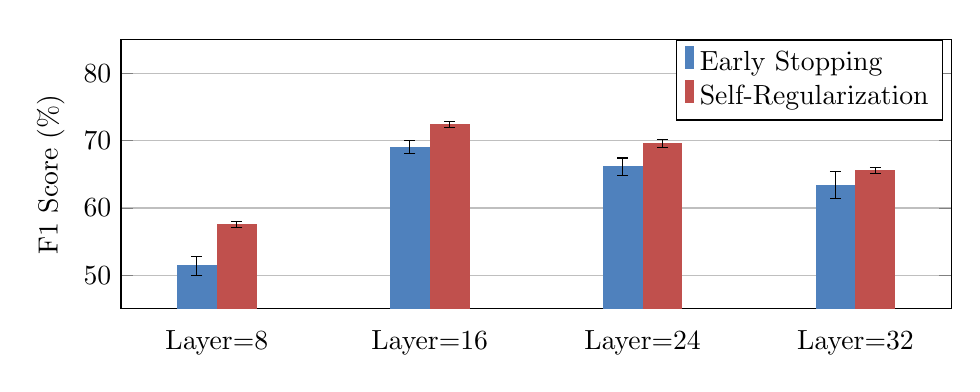
\begin{tikzpicture}
    \begin{axis}[
        width  = 1.*\linewidth,
        height = 5.0cm,
        major x tick style = transparent,
        ybar=\pgflinewidth,
        bar width=14pt,
        ymajorgrids = true,
        ylabel = {F1 Score (\%)},
        symbolic x coords={Layer=8,Layer=16,Layer=24,Layer=32},
        xtick = data,
        scaled y ticks = false,
        enlarge x limits=0.15,
        ymin=45,
        ymax=85,
        legend columns=1,
        legend cell align=left,
        legend style={
                at={(0.99,0.70)},
                anchor=south east,
                column sep=0ex
        }
    ]
        \addplot[style={bblue,fill=bblue,mark=none},
            error bars/.cd,
            y dir=both, % Error bar direction (both up and down)
            y explicit, % Enable explicit error values
            error bar style={black}
            ]
            coordinates {
            (Layer=8, 51.38) +- (0, 1.35) % Error value: ±1.5
            (Layer=16, 69.01) +- (0, 0.97)
            (Layer=24, 66.16) +- (0, 1.27)
            (Layer=32, 63.37) +- (0, 1.99)
        };

        \addplot[style={rred,fill=rred,mark=none},
            error bars/.cd,
            y dir=both, % Error bar direction (both up and down)
            y explicit, % Enable explicit error values
            error bar style={black}
            ]
            coordinates {
            (Layer=8, 57.52) +- (0, 0.43) % real std should be 0.23, but I enlarged it a little bit for visualization.
            (Layer=16, 72.44) +- (0, 0.44) % real std should be 0.14, but I enlarged it a little bit for visualization.
            (Layer=24, 69.64) +- (0, 0.60) 
            (Layer=32, 65.61) +- (0, 0.47) % real std should be 0.27, but I enlarged it a little bit for visualization.
        };

        \legend{Early Stopping,Self-Regularization}
    \end{axis}
\end{tikzpicture}
\vspace{-0.3cm}
    \caption{Performance of regularized classifiers by using text embeddings generated from different layers of Mistral-7B-inst (32 layers in total) on the Reward Modeling Task.}
    \label{fig:layers}
    \vspace{-0.3cm}
\end{figure}

\paragraph{\textbf{Middle layers yield optimal performance due to richer semantic representations.}}
The performance curve in Figure~\ref{fig:layers} exhibits a reverse U-shape, with both the baseline and Self-Regularization framework achieving their highest F1 scores at middle layers (e.g., Layer 16 and Layer 24). 
This trend reflects the richer and more task-relevant semantic information encoded in intermediate layers of the Mistral-7B model, aligned with findings from previous work~\cite{wu2024language}. 
As the baseline achieves its peak performance at Layer 16, we conduct all experiments using embeddings from this layer.

\begin{figure}
    \centering
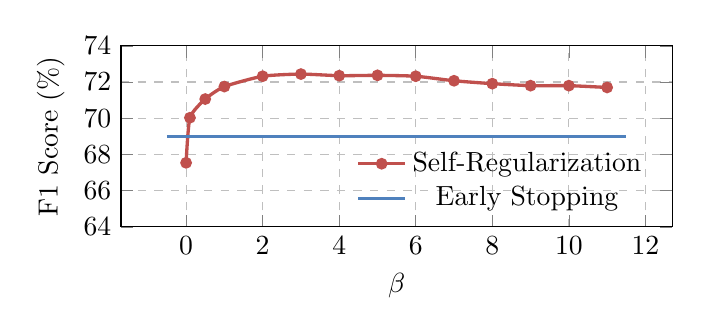
\begin{tikzpicture}
    \begin{axis}[
        xlabel={$\beta$},
        %xlabel style={yshift=-0.cm}
        ylabel={F1 Score (\%)},
        ylabel style={anchor=south},
        legend pos=south east,
        ymin=64,
        ymax=74,
        grid=major,
        grid style={dashed,gray!30},
        major grid style={lightgray},
        legend style={draw=none, fill=none},
        x tick label style={
            /pgf/number format/fixed,
            /pgf/number format/precision=3
        },
        scale only axis,
        width=7.cm,
        height=2.3cm,
    ]
    
    % Add your data points for the line plot
    
    \addplot[color=rred, smooth,tension=0.35, mark=*, 
            mark options={solid, mark size=1.5pt},
            line width=1.2pt] coordinates {
        (0.0, 67.54)
        (0.1, 70.03)  
        (0.5, 71.06)
        (1.0, 71.75) %6.78720 I adjust it a little bit for better visualization
        (2.0, 72.32)
        (3.0, 72.44)
        (4.0, 72.35)
        (5.0, 72.37)
        (6.0, 72.32)
        (7.0, 72.07)
        (8.0, 71.91)
        (9.0, 71.80)
        (10.0, 71.80)
        (11.0, 71.70)
    };
    \addlegendentry{Self-Regularization}
    \addplot[color=bblue, line width=1.0pt, mark=none, line width=1.2pt] 
        coordinates {(-0.5, 69.01) (11.5, 69.01)};
    \addlegendentry{Early Stopping}
    \end{axis}
    \end{tikzpicture}
    \vspace{-0.5cm}
    \caption{Performance of regularized classifiers with different hyper-parameters $\beta$ on the Reward Modeling task.}
    \label{fig:sensitivity_lambda}
    \vspace{-0.35cm}
\end{figure}


\paragraph{\textbf{Self-Regularization is robust to embeddings from different LLM layers $l$.}} 
Figure~\ref{fig:layers} shows that classifiers trained with the proposed framework consistently outperform the baseline across all tested layers. Although the absolute F1 scores vary by layer, the relative improvement achieved by self-regularization remains significant, demonstrating the framework's robustness to hidden representations derived from different layers.


\paragraph{\textbf{Self-Regularization demonstrates robustness to the hyper-parameter $\beta$.}}
Figure~\ref{fig:sensitivity_lambda} illustrates that the proposed method consistently achieves an F1 score of at least 70.0\% on the Reward Modeling Task across a wide range of $\beta$ values, significantly outperforming the baseline ``Early STopping'' at 69.01\%. Notably, when $\beta$ is set between 0.75 and 6.0, the method maintains peak performance, with the highest F1 score of approximately 72.44\% achieved at $\beta = 3.0$. This observation indicates that the proposed framework is stable and not overly sensitive to the choice of $\beta$.




\section{Related Works}
Our work builds on research in LLM interpretability and classifier regularization. Efforts to explain LLMs have leveraged activation monitoring~\citep{wang2023label}, probing~\citep{belinkov2018evaluating,jawahar2019does,rogers2021primer}, and basis decomposition~\citep{elhage2022toy,olah2020zoom} to address neuron polysemanticity~\cite{arora2018linear}. Recent advances use sparse autoencoders~\citep{brickentowards,cunningham2023sparse} to extract monosemantic features, improving interpretability and enabling control over model behaviors, with applications extending to translation~\citep{dumas2024llamas}, circuit detection~\citep{marks2024sparse}, and scaling to larger LLMs~\citep{templeton2024scaling,gao2024scaling,lieberum2024gemma}. We extend this line by fine-tuning sparse autoencoders on domain data to mitigate dead neurons and enhance task-specific feature reconstruction. In classifier regularization, traditional methods like weight decay~\citep{hoerl1970ridge} and dropout~\citep{srivastava2014dropout} prevent overfitting, while modern approaches such as spectral normalization~\citep{yoshida2017spectral} and focal loss~\citep{ross2017focal} refine model generalization. Our work differs by leveraging sparse autoencoders to achieve semantical regularization on embedding-based classifier training. 
Appendix~\ref{appd:related_work} provides more discussions on related works.

\section{Conclusion}
This paper introduces a framework that regularizes the usage of unintended features for embedding-based text classifiers. 
Our approach identifies unintended features within LLM-generated embeddings with sparse autoencoders, and regularizes their impact for classification by introducing a constraint loss. Empirical evaluations across three challenging text classification tasks demonstrate that our method effectively reduces unintended feature reliance and improves the generalizability of classifiers. 
This work steps a solid stamp toward controllable embedding-based text classification. 


\bibliographystyle{ACM-Reference-Format}
\bibliography{custom}


%%
%% If your work has an appendix, this is the place to put it.
\newpage
\appendix

\section{Minimum Sample Size to Effectively Estimate Mean of Sparse Feature Activations}  
\label{appd:training_size}
In this section, we aim to quantify the minimum number of training samples required to obtain a reliable estimate of the average activation values $\mathbf{A}=\sigma(\mathbf{X}\cdot\mathbf{W})$ of learned sparse features from sparse autoencoders. With the sparse nature of these learned features, we assume that each learned sparse feature is activated with probability $p$ within an input text $x$, and when activated, the value falls a normal distribution $ \mathcal{N}(\mu,\sigma^2)$, the estimation of $\mu$ requires a sufficient number of nonzero activations $n_\text{sparse}$. 
Formally, the activations of sparse features follow a Bernoulli-Gaussian distribution:
\begin{equation}
    \mathbf{A} =
\begin{cases}
Z, & \text{with probability } p, \\
0, & \text{with probability } 1 - p,
\end{cases}
\end{equation}
where $Z\sim \mathcal{N}(\mu,\sigma^2)$. 
The key challenge in estimating $\mu$ arises from the sparsity induced by $p$, which effectively reduces the number of informative samples (the values are greater than 0).

To determine the minimum required training samples $n_\text{sparse}$, we recall that the effective sample size $n_\text{normal}$ to estimate the mean of a normal distribution with a margin of error $d$ at confidence level $1-\alpha$ is given by the Central Limit Theorem~\cite{fischer2011history} as:
\begin{equation}
    n_\text{normal} = \left( \frac{z_{\alpha/2} \cdot \sigma}{d} \right)^2,
\end{equation}
where $z_{\alpha/2}$ is the z-score corresponding to the significance level $\alpha$ under a normal distribution.
However, since only a fraction $p$ of the total samples yield nonzero activations, the expected number of usable samples is $p\cdot n_\text{normal}$. Therefore, the sample size for estimating the mean activations of sparse features is adjusted as:
\begin{equation}
    n_\text{sparse} = \frac{1}{p} \left( \frac{z_{\alpha/2}\cdot \sigma}{d} \right)^2.
\end{equation}
This result highlights the influence of feature sparsity: as $p$ decreases, the total number of required samples grows proportionally as $1/p$.
In practice, if a task-specific feature occurs with a probability $p=0.01$ in the documents (which is already an ideal situation), estimating the mean activation within a margin $d=0.1\times \sigma$ at a 95\% confidence level would require approximately: 
\begin{equation}
    n_\text{sparse} = \frac{1}{0.01} \left( \frac{1.96\times \sigma}{0.1\times \sigma} \right)^2 \approx 38416.
\end{equation} 
Given that real-world datasets~\cite{wang2018glue} usually consist of thousands of training samples, which is significantly smaller than $n_\text{sparse}\approx 38416$, effectively estimating the average activations $\mathbf{A}$ of the learned sparse feature is infeasible in practice. 




\section{Details of Training Sparse Autoencoders}
\label{appd:training_sae}

\subsection{Pre-training Sparse Autoencoders.} 
The pre-training process and hyperparameter configuration adhere to established practices outlined in prior research~\citep{brickentowards,gao2024scaling,lieberum2024gemma}. For pre-training, we curated data from diverse instruction-tuning datasets, including ShareGPT~\citep{shareGPT}, UltraChat~\citep{ding2023enhancing} (randomly sampling 400,000 instances), HH-RLHF~\citep{bai2022training}, WebGLM-QA~\citep{liu2023webglm}, Evol-Instruct~\citep{xu2023wizardlm}, and HelpSteer2~\citep{wang2024helpsteer2}, while removing duplicate prompts to produce a total of approximately 711,000 unique queries spanning various topics and intents. This dataset was split into training (90\%) and validation (10\%) sets, yielding around 113 million tokens for training and 12 million tokens for validation, with an average query length of approximately 178 tokens. We initialize the sparse autoencoder with $2^{16}$ feature vectors using Kaiming initialization~\citep{he2015delving}, selecting this number based on the scaling law, i.e., $C = \mathcal{O}(Z^\gamma)$, between the feature count $C$ and the training tokens $Z$ observed in~\cite{gao2024scaling}, with $\gamma \approx 0.60$ for GPT2-small, $\gamma \approx 0.65$ for GPT-4, and $\gamma \approx 0.5978$ in our analysis. We also set Top-$K=20$ feature vectors used for each inference following previous work~\cite{gao2024scaling}. The sparse autoencoder is trained with AdamW~\cite{loshchilov2017fixing} using a constant learning rate $1e^{-3}$ and $\epsilon=6.25e^{-10}$ as suggested by~\cite{gao2024scaling}. We train the sparse autoencoder over five epochs on the pre-training dataset with a batch size of 512 prompts. 


\subsection{Fine-tuning Sparse Autoencoders.} 
We fine-tune the pre-trained sparse autoencoder on the training dataset of each task. 
At the beginning of each fine-tuning epoch, we use all feature vectors to go through the entire dataset and monitor those feature vectors that have not been activated as dead neurons. 
The Top-$K=20$ dead feature vectors are asked to reconstruct the residuals of text representations with $\alpha=0.1$. 
Fine-tuning is performed using the AdamW~\cite{loshchilov2017fixing} optimizer with $\epsilon=6.25 \times 10^{-10}$, $\beta_1=0.9$, and $\beta_2=0.999$. 
For the Toxic Chat Detection and Reward Modeling tasks, fine-tuning is conducted for a total of 5 epochs with a batch size of 512 and a learning rate of $5 \times 10^{-5}$. 
In contrast, for the Disease Diagnosis task, fine-tuning runs for 40 epochs with a batch size of 8 and a learning rate of $3 \times 10^{-6}$, as the training dataset is significantly smaller than those of the other two tasks.

\section{Details of Identifying Unintended Features}
\label{appd:interpret_sae}
\subsection{Interpreting Learned Features}
Building on prior work in LLM-as-a-judge~\citep{bills2023language,chaudhary2024evaluating,gao2024scaling,lieberum2024gemma}, we interpret the learned feature vectors from fine-tuned sparse autoencoders by identifying the Top-10 text spans that most activate each feature, with each span limited to a maximum of 32 tokens. To summarize the underlying patterns of these activations, we employ GPT-4o-mini\footnote{https://platform.openai.com/docs/guides/gpt} as our machine annotator, specifically using the gpt-4o-mini-2024-07-18 model with a temperature of 0 for deterministic decoding. Each generated response is capped at 1024 tokens. 

To enhance the reliability of automatic interpretations, we design a structured prompting framework that incorporates a role-playing strategy and in-context examples. Following previous work~\citep{bills2023language}, our machine annotator has the option to respond with "Cannot Tell" if it detects no meaningful patterns among the activated text spans. Additionally, to mitigate hallucinations, we prompt the LLM in a separate thread to verify whether its previously generated summary accurately reflects the underlying data. The complete prompting templates for summarization and verification are shown in Template 1 and Template 2, respectively. 


\begin{tcolorbox}[width=0.99\linewidth,breakable,colback=gray!5!white,colframe=blue!75!black,title=Template-1: Summarizing most activated text spans.]
\textbf{System:} You are studying a neural network. Each neuron looks for one particular concept/topic/theme/behavior/pattern. Look at some spans the neuron activates for and guess what the neuron is looking for. Pay more attention to the [last few words] of each spans in the front as they are supposed to be more correlated to the neuron behavior. Ignore the [MASK] patterns in the spans. Don't list examples of 
spans and keep your summary as detailed as possible. If you cannot summarize most of the spans, you should say "Cannot Tell."

\,


\textbf{User:} Span 1: w.youtube.com/watch?v=5qap5aO4z9A

Span 2: youtube.come/yegfnfE7vgDI

Span 3: \{'token': 'bjXRewasE36ivPBx

Span 4: /2023/fid?=0gBcWbxPi8uC

\textbf{Agent:} Base64 encoding for web development.


\,

\textbf{User:} Span 1: cross-function[MASK]

Span 2: cross-function

Span 3: [MASK][MASK] cross-function

\textbf{Agent:} Particular phrase 'cross-function'. 

\,

\textbf{User:} Span 1: novel spectroscopic imaging platform

Span 2: and protein evolutionary network modeling

Span 3: reactions-centric biochemical model

Span 4: chaperone interaction network

\textbf{Agent:} Biological terms.

\,

\textbf{User:} Span 1: is -17a967

Span 2: what is 8b8 - 10ad2

Span 3: 83 -11111011001000001011

Span 4: is -c1290 - -1

\textbf{Agent:} Synthetic math: Arithmetic, numbers with small digits, 
in unusual bases.

\,

\textbf{User:} \textit{\{Insert Most Activated Text Span Here\}}
\end{tcolorbox}

\begin{tcolorbox}[width=0.99\linewidth,breakable,colback=gray!5!white,colframe=blue!75!black,title=Template-2: Verifying automated summaries.]
\textbf{System:} You are a linguistic expert. Analyze whether the text spans 
well represents the concept/topic/theme/pattern. Organize your final 
decision in the format of "Final Decision: [[Yes/Probably/Maybe/No]]".

\,

\textbf{User:} Concept/Topic/Theme/Pattern: \{Insert Automated Summary Here\}.

Spans: \{Insert Most Activated Text Span Here\}.
\end{tcolorbox}


\subsection{Identifying Unintended Features}
For all three tasks, we define unintended features as those that lack a clear semantic correlation with the task, as determined by human-crafted evaluation rubrics. Specifically, we reference prior work to establish these rubrics: toxic detection follows~\citep{dubey2024llama3herdmodels}, reward modeling is based on~\citep{ouyang2022training}, and disease diagnosis adheres to guidelines from~\citep{xu2019end}. 
To assess feature-task relevance, we adopt the annotation framework from~\citep{lieberum2024gemma}, where the machine annotator classifies correlations into four levels: ``Yes'', ``Probably'', ``Maybe'', and ``No''. Features are considered unintended if they are not labeled as "Cannot Tell" and are assigned a task relevance level lower than ``Yes''.
For reproducibility and consistency, we provide detailed prompting templates for each task: Template 3 for toxic detection, Template 4 for reward modeling, and Template 5 for disease diagnosis.

\begin{tcolorbox}[width=0.99\linewidth,breakable,colback=gray!5!white,colframe=blue!75!black,title=Template-3: Judging relevance to Toxic Detection task.]
\textbf{System:} You are a linguistic expert. \textbf{Your job is to identify some text-based features whether they can be used to judge whether the user's intention is harmful, according to the following Guideline of User Harmfulness.} You are given the feature with its name and several text spans from the user queries as examples. Provide a short analysis on whether the feature could be used to judge the harmfulness of the user intentions. Note that, the duplicated text spans in the example are acceptable. Please do not be too mean but be as objective as possible. Organize your final decision in the format of ``Final Decision: [[ Yes/Probably/Maybe/No ]]``.

\,

\textbf{Guideline of User Harmfulness}

* The feature does not need to satisfy all the following rules.

* The feature shows that the user tries to behave in violent/non-violent crimes, including: (1) unlawful violence toward people, (2) unlawful violence toward animals, (3) personal crimes (ex: labor trafficking, threats), (4) financial crimes, (5) property crimes (theft, arson, vandalism), (6) drug crimes, (7) weapons crimes, and (8) cyber crimes (ex: hacking).

* The feature shows that the user tries to behave in sex-related crimes, including: (1) sex trafficking, (2) sexual assault (ex: rape), (3) sexual harassment (physical, verbal, or visual), (4) prostitution, and (5) sexual abuse of children.

* The feature shows that the user tries to defame others.

* The feature shows that the user tries to steal or violate intellectual property rights of others.

* The feature shows that the user tries to request privacy information from others.

* The feature shows that the user demean or dehumanize others based on their personal characteristics (i.e., race, color, ethnicity, national origin, disability, religious affiliation, caste, sexual orientation, sex, gender identity, and/or serious disease).

* The feature shows that the user has the intention of self-harm, including: (1) suicide, (2) self-injury (ex: cutting), and (3) disordered eating.

* The feature shows that the user tries to find erotic contents.


\,


\textbf{User:} Concept/Topic/Theme/Pattern: \{Insert Automated Summary Here\}.

Spans: \{Insert Most Activated Text Span Here\}.
\end{tcolorbox}

\begin{tcolorbox}[width=0.99\linewidth,breakable,colback=gray!5!white,colframe=blue!75!black,title=Template-4: Judging relevance to Reward Modeling task.]
\textbf{System:} You are a linguistic expert. \textbf{Your job is to identify some text-based features whether they can be used to judge the helpfulness of a chatbot, according to the following Guideline of Helpfulness.} You are given the feature with its name and several text spans from a user-chatbot conversation as examples. Provide a short analysis on whether the feature could be used to judge the helpfulness of the chatbot. Note that the duplicate text spans in the example are acceptable. Please do not be too mean but be as subjective as possible. Organize your final decision in the format of ``Final Decision: [[ Yes/Probably/Maybe/No ]]``. 

\,

\textbf{Guideline of Helpfulness}

* The feature does not need to satisfy all the following rules.

* The feature shows that the chatbot can write in clear and polite language.

* The feature shows that the chatbot can answer a challenging question from a user (e.g., programming, reasoning, solving math problems).

* The feature shows that the chatbot is sensitive to internationality (e.g., "football" should not mean American football, and "the president" does not necessarily mean the US president).

* The feature shows that the chatbot knows to ask for clarification if a user question is too confusing.

* The feature shows that the chatbot will not give overly long or rambling answers.

* The feature shows that the chatbot is knowledgeable in world-wide knowledge.

* The feature should not come from the user query.

\,


\textbf{User:} Concept/Topic/Theme/Pattern: \{Insert Automated Summary Here\}.

Spans: \{Insert Most Activated Text Span Here\}.
\end{tcolorbox}


\begin{tcolorbox}[width=0.99\linewidth,breakable,colback=gray!5!white,colframe=blue!75!black,title=Template-5: Judging relevance to Disease Diagnosis task.]
\textbf{System:} You are an experienced doctor. \textbf{Task: Check if the given feature and some of its example text spans show any symptoms related to the diagnosis of Upper Respiratory Tract Infection (URTI), according to the Diagnosis Guideline.} You are given the feature with its name and several text spans from some patient-doctor conversations as examples. Provide a short analysis of whether the feature connects with the diagnosis of URTI. Note that, the duplicate text spans in the example are acceptable. Please be as objective as possible. Organize your final decision in the format of ``Final Decision: [[ Yes/Probably/Maybe/No ]]``.

\,

\textbf{Diagnosis Guideline}

* The feature does not need to satisfy all the following symptoms.

* The feature shows that the patient has a fever.

* The feature shows that the patient has nasal congestion, runny nose, sneezing, cough, phlegm, and/or hoarseness.

* The feature shows that the patient feels pains in their face, head, sore throat, ears, and/or eyes.

* The feature shows that the patient feels tired or sweating. 

\,

\textbf{User:} Concept/Topic/Theme/Pattern: \{Insert Automated Summary Here\}.

Spans: \{Insert Most Activated Text Span Here\}.
\end{tcolorbox}



\section{Extended Case Studies}
\label{appd:case_study}
In this section, we provide additional qualitative analyses of the intended and unintended features identified in the Reward Modeling and Disease Diagnosis tasks. Our goal is to further illustrate the interpretability of the features learned by sparse autoencoders and how LLMs can aid in their regularization. These extended case studies highlight the effectiveness of our approach in interpreting LLM-extracted features across diverse tasks.

\subsection{Case Study on Reward Modeling Task}
Table~\ref{tab:qualitative} provides an extended qualitative analysis of LLM-identified intended and unintended features for the Reward Modeling task. In this task, the classifier predicts the helpfulness of a chatbot's responses to users. Unintended features are defined as those that are not semantically aligned with the goal of classifying helpfulness. The analysis leverages GPT-4o-mini to summarize the most activated text spans and assess their relevance to the task.

A particularly noteworthy example is the second feature, where the raw explanations highlight a diverse range of cultural references, including Japanese mayonnaise, Ugandan cuisine (Katogo), and video games like Diablo II and Spyro. According to the human-crafted helpfulness guideline (see Template-4), features showcasing the chatbot's global knowledge are considered relevant, and the LLM identifies this feature as intended. Similarly, the third feature—focused on numerical values and conversions—is deemed relevant due to its indication of the chatbot’s mathematical capabilities, which align with helpfulness criteria.

Conversely, other features such as the fourth example (focused on repetitive phrases like “over the”) are identified as unintended, as they lack meaningful semantic alignment with the task. These observations underscore the capability of LLMs to effectively distinguish between intended and unintended features, leveraging human-crafted rubrics and raw textual explanations, matching our findings from the Toxic Detection task. %This highlights the scalability of using LLMs to identify and regulate unintended features across diverse tasks.



\begin{table*}[t]
\small
    \centering
    \caption{Additional qualitative analysis on LLM-identified intended/unintended features for the Reward Modeling task, where the classifier predicts the helpfulness of a chatbot's response to the user. We \colorbox{pink}{highlight} phrases in the text spans that are semantically correlated to helpful behaviors, such as ``being polite'', ``considering diverse cultures'', and ``solving math problems''.}
    \label{rm_case_study}
    \vspace{-0.3cm}
    \begin{tabular}{p{11.0cm}|p{4.0cm}|c}
        \toprule
        \toprule
        \centering
        \textbf{Most Activated Text Spans} & \textbf{Summary of Text Spans} & \textbf{Helpful Relevant} \\
         \midrule
        \textbf{Span  1:} \_[BOT]:\_\_ \colorbox{pink}{It could}; \textbf{Span 2:} \_\_ \colorbox{pink}{Is it possible} that your symptoms could be related; \textbf{Span 4:} \_\_[BOT]:\_\_ \colorbox{pink}{Perhaps} there’s; \textbf{Span 4:} BOT]:\_\_ Good question! \colorbox{pink}{It might be}; \textbf{Span 5:} [BOT]:\_\_ Do you think \colorbox{pink}{it might}; \textbf{Span 6:} s a possibility of damage, but it \colorbox{pink}{could also}; \textbf{Span 7:} BOT]:\_\_ If you are, \colorbox{pink}{you might}; \textbf{Span 8:} n\_\_[BOT]:\_\_ \colorbox{pink}{Maybe} you’; \textbf{Span 9:} n\_\_[BOT]:\_\_ It \colorbox{pink}{could be}; \textbf{Span 10:} \_\_[BOT]:\_\_ \colorbox{pink}{Could it} & Expressing a possibility or uncertainty. & \multirow{5}{*}{Yes}\\ \hline
        \textbf{Span 1:}  a \colorbox{pink}{Japanese} mayonnaise called “Nozaw; \textbf{Span 2:}  is popularly served with \colorbox{pink}{Katogo} (beef; \textbf{Span 3:} ame, \colorbox{pink}{Spyro}: Year of the Dragon; \textbf{Span 4:}  upgrade pack called \colorbox{pink}{Diablo II}: Lord of Dest; \textbf{Span 5:}  two hours after giving the infant iron-containing; \textbf{Span 6:}  also listen to \colorbox{pink}{George Harrison’s} "My Sweet; \textbf{Span 7:} ina is \colorbox{pink}{Tina Turner’s} autobiography; \textbf{Span 8:}  model name, for example the 901; \textbf{Span 9:} I suggest looking for pieces called \colorbox{pink}{Goldberg Vari}; \textbf{Span 10:}  a message like “The bear ate the gummy & The provided text Spans contain references to diverse cultural items (Japanese mayonnaise), food (Katogo), and video games (Spyro: Year of the Dragon, Diablo II: Lord of Destruction). &  \multirow{7}{*}{Yes}\\ \hline
        \textbf{Span 1:}  day will be \colorbox{pink}{24 hours}, 1; \textbf{Span 2:}  \colorbox{pink}{20 years}, you will have \$1; \textbf{Span 3:}  \colorbox{pink}{37 degrees Fahrenheit = 3}; \textbf{Span 4:}  Sure. \colorbox{pink}{3.5 rounded up} is ; \textbf{Span 5:}  \colorbox{pink}{37 degrees Fahrenheit = 3} & The feature captures numerical values and conversions. & \multirow{2}{*}{Yes}\\ \hline
        \textbf{Span 1:}  Was considering; \textbf{Span 2:}  I'm thinking of getting; \textbf{Span 3:}  I was thinking about getting; \textbf{Span 4:}  I'm thinking about getting; \textbf{Span 5:}  What should I look for; \textbf{Span 6:}  Why are there; \textbf{Span 7:}  What things should I look for; \textbf{Span 8:}  Should I get; \textbf{Span 9:}  I'm trying to decide whether; \textbf{Span 10:}  How do I decide between getting & The feature captures user general queries. & \multirow{4}{*}{No}\\ \hline
        \textbf{Span 1:} You repeat this several times over the; \textbf{Span 2:}  “domesticated” have been selected over the; \textbf{Span 3:}  have identified over 50 million deaths during the; \textbf{Span 4:}  has been visited by nearly thirty million people over the; \textbf{Span 5:}  public areas that are increasingly crowded and busy over the; \textbf{Span 6:}  decade to actually make any progress.  Over the; \textbf{Span 7:}  other unnecessary toxins that build up over the; \textbf{Span 8:}  about 80\% of the population over the; \textbf{Span 9:}  area, though, I would estimate that over the; \textbf{Span 10:}  but rather a style of music that evolved over the & The feature captures a specific phrase ``over the''. & \multirow{5}{*}{No}\\ 
        \bottomrule
        \bottomrule
    \end{tabular}
    \label{tab:qualitative}
   % \vspace{-0.4cm}
\end{table*}

\subsection{Case Study on Disease Diagnosis Task}
For the Disease Diagnosis task, the classifier aims to determine whether a patient is suffering from either Upper Respiratory Tract Infection (URTI) or Pneumonia. Table~\ref{dd_case_study} provides a detailed analysis of LLM-identified intended and unintended features, focusing on text spans most activated by learned feature vectors. In this task, unintended features are defined as those that are not semantically correlated with the symptoms relevant to these two diseases, such as “coughing,” “fever,” and “breathing difficulties.”

One notable example is the first feature, where the raw text spans describe respiratory symptoms, including coughing, fever, and a runny nose. The LLM identifies this feature as relevant since these symptoms align directly with URTI and Pneumonia diagnoses. Similarly, the second feature, which highlights medical symptoms such as rashes, breathing difficulties, and fever in children, is classified as relevant due to its strong correlation with the target conditions.
On the other hand, features like the third example—concerning general health-related inquiries, such as asking about dietary advice or side effects from medication—are deemed irrelevant to the disease diagnosis task. Likewise, the fourth example, which describes skin conditions like red spots or rashes unrelated to respiratory issues, is identified as unintended, as it does not pertain to the symptoms of URTI or Pneumonia.

These findings demonstrate the ability of LLMs to effectively distinguish between disease-relevant and irrelevant features based on human-crafted rubrics and textual explanations. This automated process not only aids in enhancing interpretability but also highlights the potential for scalable identification of unintended features in medical classification tasks.


\begin{table*}[t]
\small
    \centering
    \caption{Additional qualitative analysis on LLM-identified intended/unintended features for the Disease Diagnosis task, where the classifier predicts whether the patient is suffering from either URTI or Pneumonia. We \colorbox{pink}{highlight} phrases in the text spans that are semantically correlated to the symptoms of these two diseases, such as ``coughing'', ``chest pains'', and ``fever''.}
    \label{dd_case_study}
    \vspace{-0.3cm}
    \begin{tabular}{p{11.0cm}|p{4.0cm}|c}
        \toprule
        \toprule
        \centering
        \textbf{Most Activated Text Spans} & \textbf{Summary of Text Spans} & \textbf{Disease Relevant} \\
         \midrule
          \textbf{Span 1:}  her head and neck. She occasionally \colorbox{pink}{coughs} a; \textbf{Span 2:}  next day, \colorbox{pink}{fever} subsided, but after a; \textbf{Span 3:}  has been \colorbox{pink}{coughing severely} for the past; \textbf{Span 4:}  but she has been \colorbox{pink}{drowsy} for the past; \textbf{Span 5:} the baby had a \colorbox{pink}{runny nose} a & Symptoms of illness, particularly respiratory symptoms like coughing and fever. &  \multirow{3}{*}{Yes}\\ \hline
          \textbf{Span 1:} Patient: The child has a rash.; \textbf{Span 2:} The baby has been \colorbox{pink}{having difficulty breathing} recently.; \textbf{Span 3:}  was found that the child indeed \colorbox{pink}{had a fever}.; \textbf{Span 4:} Patient: The baby has a \colorbox{pink}{rash}.; \textbf{Span 5:}Patient: The child is \colorbox{pink}{losing appetite}.; \textbf{Span 6:} The child has a \colorbox{pink}{rash} now.; \textbf{Span 7:}  Yes, the child has symptoms of \colorbox{pink}{breathing difficulty}.; \textbf{Span 8:}  child has had a \colorbox{pink}{cough with phlegm}.; \textbf{Span 9:}  child indeed had a \colorbox{pink}{cough with phlegm}.; \textbf{Span 10:} The baby is having \colorbox{pink}{breathing difficulties}. & Medical symptoms related to children, specifically focusing on conditions like rashes, breathing difficulties, fever, and coughs.  & \multirow{5}{*}{Yes} \\ \hline
         \textbf{Span 1:} -term, and will it have a negative impact; \textbf{Span 2:}  ask the doctor, can adult noodles possibly; \textbf{Span 3:}  mollusks in recent days, could these; \textbf{Span 4:}  and I gave her medication, which caused her; \textbf{Span 5:}  taken for nearly a week, and during which,; \textbf{Span 6:}  being bitten by mosquitoes, there; \textbf{Span 7:}  not sure if the allergy will worsen; \textbf{Span 8:}  used the laxative, and after using it & Health-related concerns and inquiries about medical conditions or treatments. &  \multirow{4}{*}{No}\\ \hline
         \textbf{Span 1:}  and a rash was found on the back,; \textbf{Span 2:}  her limbs and feet, but not on her; \textbf{Span 3:}  are rashes on the mouth, limbs,; \textbf{Span 4:}  and now there are many blisters on his; \textbf{Span 5:} , no fever. There are red spots on my; \textbf{Span 6:}  covered with small dots all over, on her; \textbf{Span 7:}  after a while, currently they are mainly on his; \textbf{Span 8:}  when held, later he could only sleep with his; \textbf{Span 9:}  had red spots on her; \textbf{Span 10:}  these red spots on the body, especially on the & Symptoms related to skin conditions, specifically rashes and spots on various body parts. & \multirow{5}{*}{No} \\

        \bottomrule
        \bottomrule
    \end{tabular}
    \label{tab:qualitative}
   % \vspace{-0.4cm}
\end{table*}


\section{Extended Related Work}
\label{appd:related_work}
In this section, we review literature related to explaining LLMs and designing regularization for embedding-based classifiers. 

\subsection{Interpreting Language Models}
Modern large language models have shown promising performance in generating texts, attracting many researchers to interpret this emergence from an internal perspective. A primary line of work~\citep{wang2023label} conducts their analysis by monitoring the differences in internal activations of input contents. 
Also, many researchers~\citep{belinkov2018evaluating,jawahar2019does,rogers2021primer} construct contrastive datasets to train a linear model for probing whether the hidden states contain a certain feature we are interested. However, this line of work is limited by the nature of the polysemantic of the neurons of deep neural networks~\cite{elhage2022toy,olah2020zoom}, meaning that this probed knowledge is too non-concise to cannot be applied for downstream tasks. To break this polysemantic barrier, some researchers~\citep{brickentowards} propose learning the basis of the activation vectors so that the (near) orthogonal property of the basis vectors could help researchers understand and even control LLM behaviors. To learn these monosemantic basis vectors, early works~\citep{Beren2022SVD,wu2024language} applies the singular vector analysis to find the main directions of the neurons spread, and they find that the explanations of these main directions are usually concise and can be used to study some general behaviors of LLMs. Soon later, sparse autoencoders~\citep{brickentowards,cunningham2023sparse} is introduced to learn the basis of the activations, which relaxes the number of basis vectors from the number of hidden dimensions to an arbitrarily large number, showing strong flexibility to study LLMs behaviors. 

Sparse autoencoders are widely used to analyze features learned by convolutional neural networks from image data~\citep{olshausen1997sparse,makhzani2013k}. However, they are still in their infancy for analyzing textual data, especially based on transformer-based language models. Researchers from Anthropic~\citep{brickentowards} and EletherAI~\cite{cunningham2023sparse} concurrently propose to study pre-trained language models with sparse autoencoders, where they show that the decomposed features from activations of small pre-trained models (such as GPT-2 and Pythia) are highly interpretable.
Many followers further investigate that these learned features can be utilized to interpret model behaviors on some easy tasks, such as the indirect object identification~\citep{makelov2024sparse}, translation~\citep{dumas2024llamas}, and circuit detection~\citep{marks2024sparse}. 
Latest works~\citep{templeton2024scaling,gao2024scaling,lieberum2024gemma} show that this technique works well with large and state-of-the-art LLMs. 
Our research follows this path and advances by leveraging the learned sparse feature vectors to develop controllable text-based classifiers. In particular, to overcome the challenge of dead neurons on the domain dataset, we propose to fine-tune a pre-trained sparse autoencoder to reconstruct residuals on the domain datasets.

\subsection{Regularizing Classifiers for Generalizability}
Regularization techniques play a critical role in improving the generalizability of classifiers by mitigating overfitting and enhancing robustness. 
The majority line of this work assumes that there is no prior knowledge of the features space, so they are widely applied to train deep neural networks. Early methods such as weight decay (L2 regularization)~\cite{hoerl1970ridge} and dropout~\cite{srivastava2014dropout} constrain model capacity or introduce stochasticity to prevent reliance on specific features. Spectral normalization~\cite{yoshida2017spectral} implicitly regularizes models by stabilizing training dynamics and controlling the Lipschitz constant, respectively. More recent advances include label smoothing~\cite{muller2019does}, which reduces overconfidence in predictions, and Focal Loss~\cite{ross2017focal} encourages the classifier to pay more attention to those hard samples. 
Our study shares the same objective as these studies, focusing on improving the generalizability of embedding-based classifiers. 
However, we achieve precise control of the classifier by first interpreting the latent space of the input representations and then regularizing the classifier based on our interpreted features.

\end{document}


\endinput
%%
%% End of file `sample-sigconf.tex'.
